% =====================================================================
% Supplementary Information for paper11_forecasting_baselines_v67
% Forecasting against naive benchmarks: a scored test of process-based
% modules on Northern cod and the Edwards Aquifer
% Part A (S1-S14): Northern cod; Part B (S15-S22): Edwards J-17;
% Part C (S23-S24): cross-system material and verification record.
% =====================================================================
\documentclass[preprint,11pt,authoryear]{elsarticle}
\usepackage{amsmath,amssymb,amsthm}
\usepackage{booktabs}
\usepackage{array}
\usepackage{tabularx}
\usepackage{longtable}
\usepackage{graphicx}
\graphicspath{{./}{figs/}{paper11_forecasting_baselines_v67_src/figs/}}
\usepackage{enumitem}
\usepackage{placeins}
\usepackage[colorlinks=true,urlcolor=blue,linkcolor=blue,citecolor=blue]{hyperref}
\emergencystretch=3em
\setlength{\tolerance}{2000}
\renewcommand{\topfraction}{0.9}
\renewcommand{\textfraction}{0.07}
\renewcommand{\floatpagefraction}{0.75}

\renewcommand{\thesection}{S\arabic{section}}
\renewcommand{\thetable}{S\arabic{table}}
\renewcommand{\thefigure}{S\arabic{figure}}
\renewcommand{\theequation}{S\arabic{equation}}
\theoremstyle{remark}
\newtheorem{remark}{Remark}
\renewcommand{\theremark}{S\arabic{remark}}

\newcommand{\kt}{\,\mathrm{kt}}
\newcommand{\Blim}{B_{\mathrm{lim}}}
\newcommand{\RMSE}{\mathrm{RMSE}}
\newcommand{\sA}{\mathfrak{s}}
\newcolumntype{L}{>{\raggedright\arraybackslash}X}

\journal{Environmental Modelling \& Software}

\begin{document}

\begin{frontmatter}
\title{Supplementary Information for:\\ Forecasting against naive benchmarks: a scored test of process-based modules on Northern cod and the Edwards Aquifer}
\author[1]{Amin Abaee\corref{cor1}}
\ead{amin_abaee@ut.ac.ir}
\cortext[cor1]{Corresponding author. ORCID: 0000-0002-0019-1842.}
\affiliation[1]{organization={Independent Researcher}, city={Tehran}, country={Iran}}
\begin{abstract}
This Supplementary Information records the material that supports the main text without carrying its argument. Part A (Northern cod): the pass order and protocol status (S1); the origin sets (S2); the full Diebold--Mariano and paired block-bootstrap grids with block-length sensitivity (S3); the period decomposition at five years and under annual landings, the fixed windows and the variant passes (S4); the fitted parameters at every window and origin (S5); the floor-forecast census (S6); the secondary scores (S7); the simulation design, its full decomposition and the alternative decision rules (S8); the decomposition of the lagged-start deficit (S9); the outcome years 2016--2021 (S10); the vintage and threshold record (S11); the 2022--2023 observation suspension (S12); the reproducibility and verification record of the cod runners (S13); and the catch-timing sensitivity (S14). Part B (Edwards J-17): the protocol record and its disclosed deviations (S15); origin sets, windows and data processing (S16); the fixed windows (S17); the two implementations of the uncertainty layer (S18); the post-2007 threshold-indicator record (S19); the service series (S20); the pumpage counterfactuals (S21); and the climate-pass fixed windows with the Uvalde note (S22). Part C: the horizon profiles of the two baselines on all three series and the autocorrelations used by Proposition~2 (S23), and the verification record for this edition (S24). Section, table and figure numbers of the main text are cited as such; sections of this document are cited as S1--S24. No archived score was changed in this edition; the computations new to it are those of S23.
\end{abstract}
\end{frontmatter}

\part*{Part A: Northern cod, NAFO 2J3KL}
\addcontentsline{toc}{part}{Part A: Northern cod}

\section{Pass order and protocol status}\label{si:passes}

The study is a fixed computational protocol with a recorded execution order, not a prospective registration: no dated pre-scoring protocol file exists for the empirical passes. The order below is established from the analysis code and its archived metadata. Passes 1 and 2 are labelled in the driver script \texttt{run\_ladder.py} and distinguished in \texttt{results/meta.json} by the keys \texttt{catch\_pass1} and \texttt{catch\_pass2}; passes 3 and 4 are separate scripts that import from that driver, which fixes their order after it.

\begin{table}[!htb]
\centering\footnotesize\setlength{\tabcolsep}{3.5pt}
\caption{Order in which the passes were run.}
\begin{tabularx}{\textwidth}{@{}clLL@{}}
\toprule
\# & Pass & Data treatment & Script / archived output \\
\midrule
1 & Coarse-regime catch & 240/120/5\,kt (through 1991 / 1992 / from 1993) & \texttt{run\_\allowbreak{}ladder.py} (pass 1); \texttt{fixed\_\allowbreak{}window\_\allowbreak{}scores.csv}, \texttt{rolling\_\allowbreak{}summary.csv} (rows \texttt{catch = regime}), \texttt{rolling\_\allowbreak{}forecasts\_\allowbreak{}regime.csv} \\
2 & Annual landings & Schijns et al.\ (2021) Table 1, t/1000 & \texttt{run\_\allowbreak{}ladder.py} (pass 2); same files, rows \texttt{catch = annual}; \texttt{rolling\_\allowbreak{}forecasts.csv} \\
2b & Survey start & Forecast initiated at the survey-scaled state, annual catch & \texttt{run\_\allowbreak{}survey\_\allowbreak{}start()} within pass 2; \texttt{survey\_\allowbreak{}start\_\allowbreak{}forecasts.csv} \\
3 & Capelin variants & Two-regime $r$ at the 1991 break; acoustic-index multiplier on observed years & \texttt{run\_\allowbreak{}capelin\_\allowbreak{}regime.py}, \texttt{run\_\allowbreak{}capelin\_\allowbreak{}index.py}; \texttt{capelin\_\allowbreak{}*\_\allowbreak{}summary.csv} \\
4 & Specification B & The ladder on the xteNCAM series alone, not pooled & \texttt{run\_\allowbreak{}xte.py}; \texttt{xte\_\allowbreak{}rolling\_\allowbreak{}summary.csv}, \texttt{xte\_\allowbreak{}fixed\_\allowbreak{}window\_\allowbreak{}scores.csv} \\
5 & Uncertainty layer & DM statistics and block bootstrap on the archived per-origin files & \texttt{campaign\_\allowbreak{}e1\_\allowbreak{}dm\_\allowbreak{}uncertainty\_\allowbreak{}regime.py}; \texttt{e1\_\allowbreak{}dm\_\allowbreak{}uncertainty\_\allowbreak{}regime.csv} \\
6 & Simulation & D1--D5 per \texttt{SPECIFICATION\_\allowbreak{}v4.md} (locked 2026-09-10 before the code was written); D6--D7 per Amendment 1 (locked 2026-09-11) & \texttt{tools/\allowbreak{}sim\_\allowbreak{}retention\_\allowbreak{}power.py}; \texttt{sim\_\allowbreak{}retention\_\allowbreak{}power.csv}, \texttt{sim\_\allowbreak{}misspecified\_\allowbreak{}D6D7.csv} \\
7 & Preceding edition & Re-execution of passes 1--6 in a third environment; paired bootstrap confirmation; period decomposition; rolling parameter record; catch-timing sensitivity & \texttt{paper11\_\allowbreak{}forecasting\_\allowbreak{}baselines\_\allowbreak{}v67\_\allowbreak{}src/\allowbreak{}work/\allowbreak{}cod/\allowbreak{}} in the repository \\
\bottomrule
\end{tabularx}
\end{table}

Three points bear on how the scores should be read. The five ladder modules were fixed before any pass was scored: the \texttt{SPECS} list in \texttt{run\_ladder.py} defines M1, M1b, M2, M3 and M4 once, Specification B imports that list rather than redefining it, and none was altered after a score was seen. The scoring core, the fixed windows, the rolling-origin RMSE comparison and the persistence bar at both horizons, was coded before the first pass. Two elements of the retention rule were formalised after the pass-1 scores had been computed: the 5\% tie band and the comparator declarations for the non-nested modules (M2 against M1, M4 against M3). Neither decides any retention outcome, the smallest pooled deficit against persistence being 17.1\%. The capelin pass is the one place where a model was added after scoring began (the index multiplier), and it is reported as a variant, not as a member of the ladder. Specification B was run last and never pooled with Specification A; the constraint is recorded in the code's docstring and in \texttt{meta.json}.

\section{Origin sets and windows}\label{si:origins}

\begin{table}[!htb]
\centering\footnotesize\setlength{\tabcolsep}{3.5pt}
\caption{Origin sets. All baselines are evaluated on the module's own origin set at each horizon. The mixed-origin persistence values that the archived Specification B summary also carries (87.6 and 317.7\,kt on 63 and 59 origins) are not comparators and are not used.}
\begin{tabularx}{\textwidth}{@{}>{\raggedright\arraybackslash}p{0.36\textwidth}Lcc@{}}
\toprule
Pass & Origins & $n$ ($h=1$) & $n$ ($h=5$) \\
\midrule
Specification A, ladder (all catch passes, survey start, two-regime $r$) & 1990--2014 ($h=1$); 1990--2010 ($h=5$); minimum eight training years & 25 & 21 \\
Specification A, capelin-index multiplier & 1991--2014; 1991--2010 (origins with a carried acoustic value) & 24 & 20 \\
Specification B, ladder and two-regime $r$ & 1965--2023; 1965--2019; minimum twelve training years & 59 & 55 \\
Specification B, capelin-index multiplier & 1988--2023; 1988--2019 & 36 & 32 \\
\bottomrule
\end{tabularx}
\end{table}

The capelin acoustic index is observed in 1982 and 1985--2023 with gaps (1983, 1984, 1993--1995, 1997, 1998, 2006, 2016, 2020--2022 missing; 2023 $= 331.3\kt$). The multiplier pass carries the last observed value across gaps and drops origins with no carried value; the two-regime pass uses the 1991 capelin collapse as a declared break and allows $r$ to differ before and after it, with the post-break value estimated only once post-break transitions are in the training window.

\FloatBarrier
\section{Uncertainty layer: full grids}\label{si:uncertainty}

Table~\ref{tab:si_dm} gives every module--benchmark pair of the archived uncertainty layer: the DM statistic (loss differences of squared errors; autocorrelation-consistent variance truncated at lag $h-1$; reported as a $z$-score), the paired moving-block bootstrap interval of the RMSE gap (block $\max(h,3)$, 20\,000 replicates, seed 0) and its two-sided $p$-value. The bootstrap in the archived script draws block indices from a generator seeded identically for the two loss series, so the resample is paired; re-running it with an explicitly shared index draw reproduces every interval to the printed digit. Table~\ref{tab:si_blocks} gives the block-length sensitivity (5\,000 replicates per cell) for the M1 and M3 persistence margins.

\begin{table}[!htb]
\centering\scriptsize
\setlength{\tabcolsep}{3.5pt}
\caption{Archived uncertainty layer: all pairs. RMSE in kt; gap $=\RMSE(A)-\RMSE(B)$; CI is the 95\% paired block-bootstrap interval of the gap; $p$ is the two-sided bootstrap $p$-value. The M2-against-M1b rows are an alternative-comparator disclosure, not part of the rule.}
\label{tab:si_dm}
\scriptsize\setlength{\tabcolsep}{2.5pt}
\begin{tabular}{@{}ccllrrrrrlr@{}}
\toprule
Spec. & $h$ & A & B & $n$ & RMSE(A) & RMSE(B) & gap & DM $z$ & 95\% CI & $p$ \\
\midrule
A & 1 & M1 & persistence & 25 & 120.5 & 98.0 & +22.5 & 1.13 & [-13.4, +52.2] & 0.19 \\
A & 1 & M1b & persistence & 25 & 114.8 & 98.0 & +16.8 & 0.98 & [-19.4, +59.6] & 0.38 \\
A & 1 & M2 & persistence & 25 & 144.1 & 98.0 & +46.0 & 1.29 & [-12.3, +83.0] & 0.45 \\
A & 1 & M3 & persistence & 25 & 134.6 & 98.0 & +36.6 & 0.99 & [-16.8, +64.2] & 0.93 \\
A & 1 & M4 & persistence & 25 & 195.6 & 98.0 & +97.5 & 1.53 & [-9.1, +172.7] & 0.28 \\
A & 1 & M2 & M1 & 25 & 144.1 & 120.5 & +23.5 & 0.91 & [-60.7, +66.9] & 0.68 \\
A & 1 & M4 & M3 & 25 & 195.6 & 134.6 & +60.9 & 1.21 & [+4.4, +134.4] & $<0.005$ \\
A & 1 & M2 & M1b & 25 & 144.1 & 114.8 & +29.3 & 0.91 & [-67.6, +82.8] & 0.70 \\
A & 5 & M1 & persistence & 21 & 288.7 & 264.7 & +24.0 & 1.84 & [-43.1, +56.4] & 0.28 \\
A & 5 & M1b & persistence & 21 & 288.6 & 264.7 & +23.9 & 1.84 & [-43.1, +56.4] & 0.28 \\
A & 5 & M2 & persistence & 21 & 398.2 & 264.7 & +133.5 & 1.10 & [-21.0, +217.5] & 0.42 \\
A & 5 & M3 & persistence & 21 & 366.4 & 264.7 & +101.6 & 1.12 & [-0.8, +151.4] & 0.08 \\
A & 5 & M4 & persistence & 21 & 488.2 & 264.7 & +223.5 & 1.14 & [-20.8, +409.4] & 0.40 \\
A & 5 & M2 & M1 & 21 & 398.2 & 288.7 & +109.5 & 0.98 & [-77.1, +232.8] & 0.81 \\
A & 5 & M4 & M3 & 21 & 488.2 & 366.4 & +121.9 & 1.15 & [-27.4, +263.2] & 0.71 \\
A & 5 & M2 & M1b & 21 & 398.2 & 288.6 & +109.7 & 0.98 & [-77.1, +232.8] & 0.81 \\
B & 1 & M1 & persistence & 59 & 119.5 & 84.4 & +35.0 & 2.81 & [+2.7, +70.8] & 0.03 \\
B & 1 & M1b & persistence & 59 & 151.6 & 84.4 & +67.2 & 3.60 & [+18.3, +117.7] & 0.01 \\
B & 1 & M2 & persistence & 59 & 166.0 & 84.4 & +81.6 & 3.22 & [+36.4, +122.8] & $<0.005$ \\
B & 1 & M3 & persistence & 59 & 126.7 & 84.4 & +42.3 & 1.85 & [+1.0, +92.5] & 0.04 \\
B & 1 & M4 & persistence & 59 & 205.7 & 84.4 & +121.3 & 3.20 & [+53.7, +193.0] & $<0.005$ \\
B & 1 & M2 & M1 & 59 & 166.0 & 119.5 & +46.6 & 1.78 & [-20.5, +104.5] & 0.17 \\
B & 1 & M4 & M3 & 59 & 205.7 & 126.7 & +79.0 & 3.07 & [+35.6, +116.4] & $<0.005$ \\
B & 1 & M2 & M1b & 59 & 166.0 & 151.6 & +14.4 & 0.51 & [-67.5, +89.1] & 0.77 \\
B & 5 & M1 & persistence & 55 & 431.9 & 300.0 & +131.9 & 2.06 & [+33.2, +218.6] & 0.01 \\
B & 5 & M1b & persistence & 55 & 445.5 & 300.0 & +145.5 & 1.80 & [+18.2, +250.9] & 0.02 \\
B & 5 & M2 & persistence & 55 & 1058.9 & 300.0 & +758.9 & 2.15 & [+363.6, +1038.5] & $<0.005$ \\
B & 5 & M3 & persistence & 55 & 930.1 & 300.0 & +630.2 & 2.39 & [+352.8, +845.6] & $<0.005$ \\
B & 5 & M4 & persistence & 55 & 1030.7 & 300.0 & +730.8 & 2.35 & [+407.3, +978.3] & $<0.005$ \\
B & 5 & M2 & M1 & 55 & 1058.9 & 431.9 & +627.0 & 1.97 & [+195.7, +929.7] & $<0.005$ \\
B & 5 & M4 & M3 & 55 & 1030.7 & 930.1 & +100.6 & 1.88 & [+20.2, +177.4] & 0.01 \\
B & 5 & M2 & M1b & 55 & 1058.9 & 445.5 & +613.4 & 1.93 & [+170.9, +945.1] & $<0.005$ \\
\bottomrule
\end{tabular}
\end{table}

\begin{table}[!htb]
\centering\scriptsize
\setlength{\tabcolsep}{2.6pt}
\caption{Block-length sensitivity of the paired bootstrap interval (kt) for the persistence margins of M1 and M3. The archived layer uses block 3 at $h=1$ and block 5 at $h=5$. One classification changes with the block: the M3 one-step margin on Specification B includes zero for blocks of four or more.}
\label{tab:si_blocks}
\scriptsize\setlength{\tabcolsep}{2.5pt}
\resizebox{\textwidth}{!}{%
\begin{tabular}{@{}cclrcccccc@{}}
\toprule
Spec. & $h$ & Module & gap & block 2 & block 3 & block 4 & block 5 & block 6 & block 8 \\
\midrule
A & 1 & M1 & +22.5 & [-13, +49] & [-13, +52] & [-14, +54] & [-16, +55] & [-18, +56] & [-18, +56] \\
A & 1 & M3 & +36.6 & [-17, +77] & [-17, +65] & [-16, +56] & [-15, +54] & [-14, +55] & [-14, +55] \\
A & 5 & M1 & +24.0 & [-37, +56] & [-37, +56] & [-41, +58] & [-43, +56] & [-51, +55] & [-65, +56] \\
A & 5 & M3 & +101.6 & [-17, +181] & [-10, +179] & [-0.4, +167] & [-0.8, +151] & [-3, +158] & [-3, +152] \\
B & 1 & M1 & +35.0 & [+5, +67] & [+2, +71] & [+1, +74] & [+1, +74] & [+0.1, +75] & [+1, +73] \\
B & 1 & M3 & +42.3 & [+4, +87] & [+1, +95] & [-1, +95] & [-3, +93] & [-4, +90] & [-4, +81] \\
B & 5 & M1 & +131.9 & [+62, +198] & [+49, +208] & [+37, +215] & [+33, +221] & [+25, +224] & [+13, +232] \\
B & 5 & M3 & +630.2 & [+436, +803] & [+394, +830] & [+362, +848] & [+348, +843] & [+310, +850] & [+272, +849] \\
\bottomrule
\end{tabular}}

\end{table}

The DM $z$-statistic is less stable than the bootstrap under the truncation lag: for the M1 persistence margin at $h=1$ it moves from 1.14 at lag 0 to 2.30 at lag 3 on Specification A and from 2.81 to 1.70 on Specification B, crossing the conventional 1.96 in opposite directions, whereas the bootstrap $p$ moves within 0.17--0.19 (A) and 0.036--0.049 (B) over blocks 3--9. Four of the 28 persistence and comparator rows have a bootstrap interval excluding zero with $|z|<1.96$ (A, $h=1$, M4 vs M3; B, $h=1$, M3 vs persistence; B, $h=5$, M1b vs persistence; B, $h=5$, M4 vs M3). No verdict rests on either statistic where they disagree; the retention rule is applied to point estimates.

\FloatBarrier
\section{Period decomposition: five-year horizon, annual pass, pooled margins}\label{si:periods}

\begin{table}[!htb]
\centering\footnotesize\setlength{\tabcolsep}{3.5pt}
\caption{Five-year rolling-origin RMSE (kt) by period of the forecast origin, with origin-matched persistence; superscripts are the number of origins at which the forecast sits at the numerical floor. Companion to Table 6.}
\label{tab:si_h5}
\begin{tabular}{@{}llrrrrrrr@{}}
\toprule
Spec. & Origins & $n$ & persist & M1 & M1b & M2 & M3 & M4 \\
\midrule
A & 1990--1995 & 6 & 479.4 & 501.1$^{4}$ & 500.8$^{4}$ & 740.0$^{1}$ & 674.5$^{3}$ & 909.2$^{1}$ \\
A & 1996--2012 & 15 & 78.6 & 127.6$^{15}$ & 127.6$^{15}$ & 54.7 & 77.1 & 54.9 \\
A & 1996--2014 & 15 & 78.6 & 127.6$^{15}$ & 127.6$^{15}$ & 54.7 & 77.1 & 54.9 \\
\midrule
B & 1965--1990 & 26 & 398.8 & 573.4$^{10}$ & 595.2$^{17}$ & 1186.2$^{7}$ & 1178.6$^{7}$ & 1252.0$^{7}$ \\
B & 1991--1995 & 5 & 301.9 & 211.2$^{4}$ & 27.5$^{5}$ & 1490.1 & 834.3$^{4}$ & 1223.5$^{3}$ \\
B & 1996--2012 & 17 & 123.3 & 178.5$^{17}$ & 178.5$^{17}$ & 250.9 & 217.3 & 217.8 \\
B & 2013--2023 & 7 & 119.9 & 367.8$^{5}$ & 406.6$^{7}$ & 1358.2 & 1012.9 & 1157.9 \\
B & 1996--2023 & 24 & 122.3 & 249.0$^{22}$ & 266.1$^{24}$ & 763.3 & 576.8 & 651.7 \\
\bottomrule
\end{tabular}
\end{table}

\begin{table}[!htb]
\centering\footnotesize\setlength{\tabcolsep}{3.5pt}
\caption{Specification A, annual-landings pass: rolling-origin RMSE (kt) by period at $h=1$ (upper block) and $h=5$ (lower block). The low-biomass band gives the same ordering as the coarse-regime pass.}
\label{tab:si_annual}
\begin{tabular}{@{}llrrrrrrr@{}}
\toprule
Spec. & Origins & $n$ & persist & M1 & M1b & M2 & M3 & M4 \\
\midrule
A & 1990--1995 & 6 & 193.6 & 209.6$^{3}$ & 187.1$^{4}$ & 325.6 & 312.1$^{3}$ & 419.1 \\
A & 1996--2012 & 17 & 19.6 & 63.0$^{12}$ & 69.9$^{13}$ & 17.2 & 15.0 & 19.8 \\
A & 2013--2014 & 2 & 66.7 & 127.2 & 134.7 & 33.5 & 28.7 & 40.2 \\
A & 1996--2014 & 19 & 28.5 & 72.5$^{12}$ & 79.2$^{13}$ & 19.6 & 17.0 & 22.9 \\
\midrule
A & 1990--1995 & 6 & 479.4 & 501.1$^{4}$ & 500.8$^{4}$ & 732.3$^{1}$ & 647.5$^{3}$ & 906.6$^{1}$ \\
A & 1996--2012 & 15 & 78.6 & 127.6$^{15}$ & 127.6$^{15}$ & 50.9 & 73.0 & 49.7 \\
A & 1996--2014 & 15 & 78.6 & 127.6$^{15}$ & 127.6$^{15}$ & 50.9 & 73.0 & 49.7 \\
\bottomrule
\end{tabular}
\end{table}

\begin{table}[!htb]
\centering\footnotesize\setlength{\tabcolsep}{3.5pt}
\caption{Post-1995 pooled margins against persistence (origins 1996 onward), with paired block-bootstrap intervals (block $\max(h,3)$, 20\,000 replicates). Specification A: 1996--2014 ($h=1$) and 1996--2010 ($h=5$); Specification B: 1996--2023 and 1996--2019. The bands were chosen after the data were seen; this table describes, it does not test.}
\label{tab:si_post1995}
\begin{tabular}{@{}cccllrrrlr@{}}
\toprule
Spec. & $h$ & $n$ & Module & RMSE & persist & gap & rel. & 95\% CI (kt) & $p$ \\
\midrule
A & 1 & 19 & M1 & 73.1 & 28.5 & +44.6 & +156\% & [+28.9, +60.3] & $<0.005$ \\
A & 1 & 19 & M1b & 79.8 & 28.5 & +51.3 & +180\% & [+28.9, +69.5] & $<0.005$ \\
A & 1 & 19 & M2 & 19.4 & 28.5 & -9.1 & -32\% & [-17.1, +6.6] & 0.47 \\
A & 1 & 19 & M3 & 16.7 & 28.5 & -11.8 & -41\% & [-20.5, +3.3] & 0.19 \\
A & 1 & 19 & M4 & 22.1 & 28.5 & -6.4 & -22\% & [-14.1, +9.0] & 0.72 \\
A & 5 & 15 & M1 & 127.6 & 78.6 & +49.0 & +62\% & [+15.4, +68.1] & $<0.005$ \\
A & 5 & 15 & M1b & 127.6 & 78.6 & +49.0 & +62\% & [+15.4, +68.1] & $<0.005$ \\
A & 5 & 15 & M2 & 54.7 & 78.6 & -23.8 & -30\% & [-27.5, +11.9] & 0.76 \\
A & 5 & 15 & M3 & 77.1 & 78.6 & -1.5 & -2\% & [-2.7, +31.7] & 0.19 \\
A & 5 & 15 & M4 & 54.9 & 78.6 & -23.6 & -30\% & [-27.2, +12.1] & 0.78 \\
B & 1 & 28 & M1 & 91.5 & 41.5 & +50.0 & +121\% & [+26.3, +78.8] & $<0.005$ \\
B & 1 & 28 & M1b & 124.0 & 41.5 & +82.5 & +199\% & [+53.2, +117.7] & $<0.005$ \\
B & 1 & 28 & M2 & 102.7 & 41.5 & +61.2 & +148\% & [-2.5, +93.3] & 0.06 \\
B & 1 & 28 & M3 & 62.3 & 41.5 & +20.9 & +50\% & [-11.1, +47.0] & 0.25 \\
B & 1 & 28 & M4 & 87.4 & 41.5 & +45.9 & +111\% & [-4.9, +73.3] & 0.08 \\
B & 5 & 24 & M1 & 249.0 & 122.3 & +126.7 & +104\% & [+27.3, +196.8] & $<0.005$ \\
B & 5 & 24 & M1b & 266.1 & 122.3 & +143.8 & +118\% & [+27.3, +227.5] & $<0.005$ \\
B & 5 & 24 & M2 & 763.3 & 122.3 & +641.0 & +524\% & [+97.9, +972.2] & $<0.005$ \\
B & 5 & 24 & M3 & 576.8 & 122.3 & +454.5 & +372\% & [+46.6, +708.8] & $<0.005$ \\
B & 5 & 24 & M4 & 651.7 & 122.3 & +529.4 & +433\% & [+61.7, +813.0] & $<0.005$ \\
\bottomrule
\end{tabular}
\end{table}

Band-level intervals for the collapse bands ($n=5$--6) are degenerate under a block bootstrap and are not reported. A leave-one-origin-out check on the Specification B collapse band confirms that the orderings there do not depend on a single origin: M1 and M1b are below persistence in all five leave-one-out sets and M3 in four of five, but these are the floor-forecast wins discussed in main-text Section 3.4.

\FloatBarrier
\subsection*{S4.1 Fixed windows (moved from the main text of the single-system edition)}

The fixed windows are diagnostic, not retention. From the 1983--1990 training window, in which SSB varied between 835 and 942\,kt, every module forecasts continuation (Table~\ref{tab:si_fixed}, Fig.~\ref{fig:si_windows}). The autonomous modules place the stock at the fitted equilibrium, 888.6\,kt, and hold it there for five years; the catch-supplied modules, told that removals fall from 240 to 120 to 5\,kt, forecast growth to about 1050\,kt by 1993. The observed path falls from 862 to 9.7\,kt. Persistence (670\,kt RMSE) is the least bad because it at least does not grow; the autonomous modules (694) are close to it, and M2--M4 (819) are the worst because the catch cut, which in reality accompanied the collapse, is read by a stock-flow model as a reason for the stock to rise. On Specification B the pattern repeats from a 36-year training window (M1 817, M1b 906, M2 1898\,kt against persistence 633).

The recovery window tells a different story. From 1995--2007, when SSB sat between 10 and 81\,kt, M1 and M2 coincide (training-mean catch and realised catch are both about 5\,kt) and over-predict the rebuild (120\,kt RMSE against 104 for persistence); M3 and M4 over-predict more (220 and 214), because the last training residual is a large positive increment ($+28\kt$ in 2006--2007) that the AR term with $\phi=0.95$ carries along the whole path. With annual landings the over-prediction is larger still (M3 609\,kt), since the fitted $K$ runs to its 5000-kt bound and production no longer saturates (Fig.~\ref{fig:si_windows_annual} in S14). The one module that beats persistence in this window, M1b (90 and 78\,kt), does so for a reason that undermines rather than supports it: its $\sA$ estimate descends to zero and its $K$ to 106--130\,kt, so it forecasts a flat line at a carrying capacity equal to the recent range. That is a persistence forecast produced by a production model whose parameters have lost their meaning (S5). On Specification B the recovery-stall window shows the same ordering: M1b 178, M1 254, M2--M4 about 268\,kt, persistence 262.

\begin{table}[!htb]
\centering\footnotesize\setlength{\tabcolsep}{3.5pt}
\caption{Fixed-window path RMSE (kt). Specification A, coarse-regime catch; the annual-landings pass and Specification B are given for the same windows. Persistence is frozen at the last training value; the training mean is the mean of the training window. Bold marks the lowest value in each column.}
\label{tab:si_fixed}
\begin{tabular}{@{}lrrrrrr@{}}
\toprule
 & \multicolumn{3}{c}{Specification A} & & \multicolumn{2}{c}{Specification B} \\
\cmidrule(lr){2-4}\cmidrule(lr){6-7}
 & collapse & recovery & recovery & & collapse & recovery stall \\
 & 1991--95 & 2008--15 & 2008--15 & & 1990--95 & 2013--24 \\
Forecaster & coarse & coarse & annual & & annual & annual \\
\midrule
persistence & \textbf{669.8} & 103.8 & 103.8 & & \textbf{632.7} & 261.7 \\
training mean & 687.9 & 144.4 & 144.4 & & 591.2 & 320.7 \\
M1 autonomous & 694.3 & 119.6 & 263.7 & & 817.3 & 254.3 \\
M1b depensatory & 693.6 & \textbf{89.8} & \textbf{78.1} & & 905.6 & \textbf{178.0} \\
M2 stock-flow & 819.4 & 119.6 & 302.8 & & 1897.7 & 268.8 \\
M3 AR residual & 819.4 & 219.7 & 609.1 & & 1767.8 & 267.7 \\
M4 lagged start & 819.1 & 214.1 & 586.3 & & 1871.9 & 268.8 \\
\bottomrule
\end{tabular}
\end{table}

\begin{figure}[!htb]
\centering
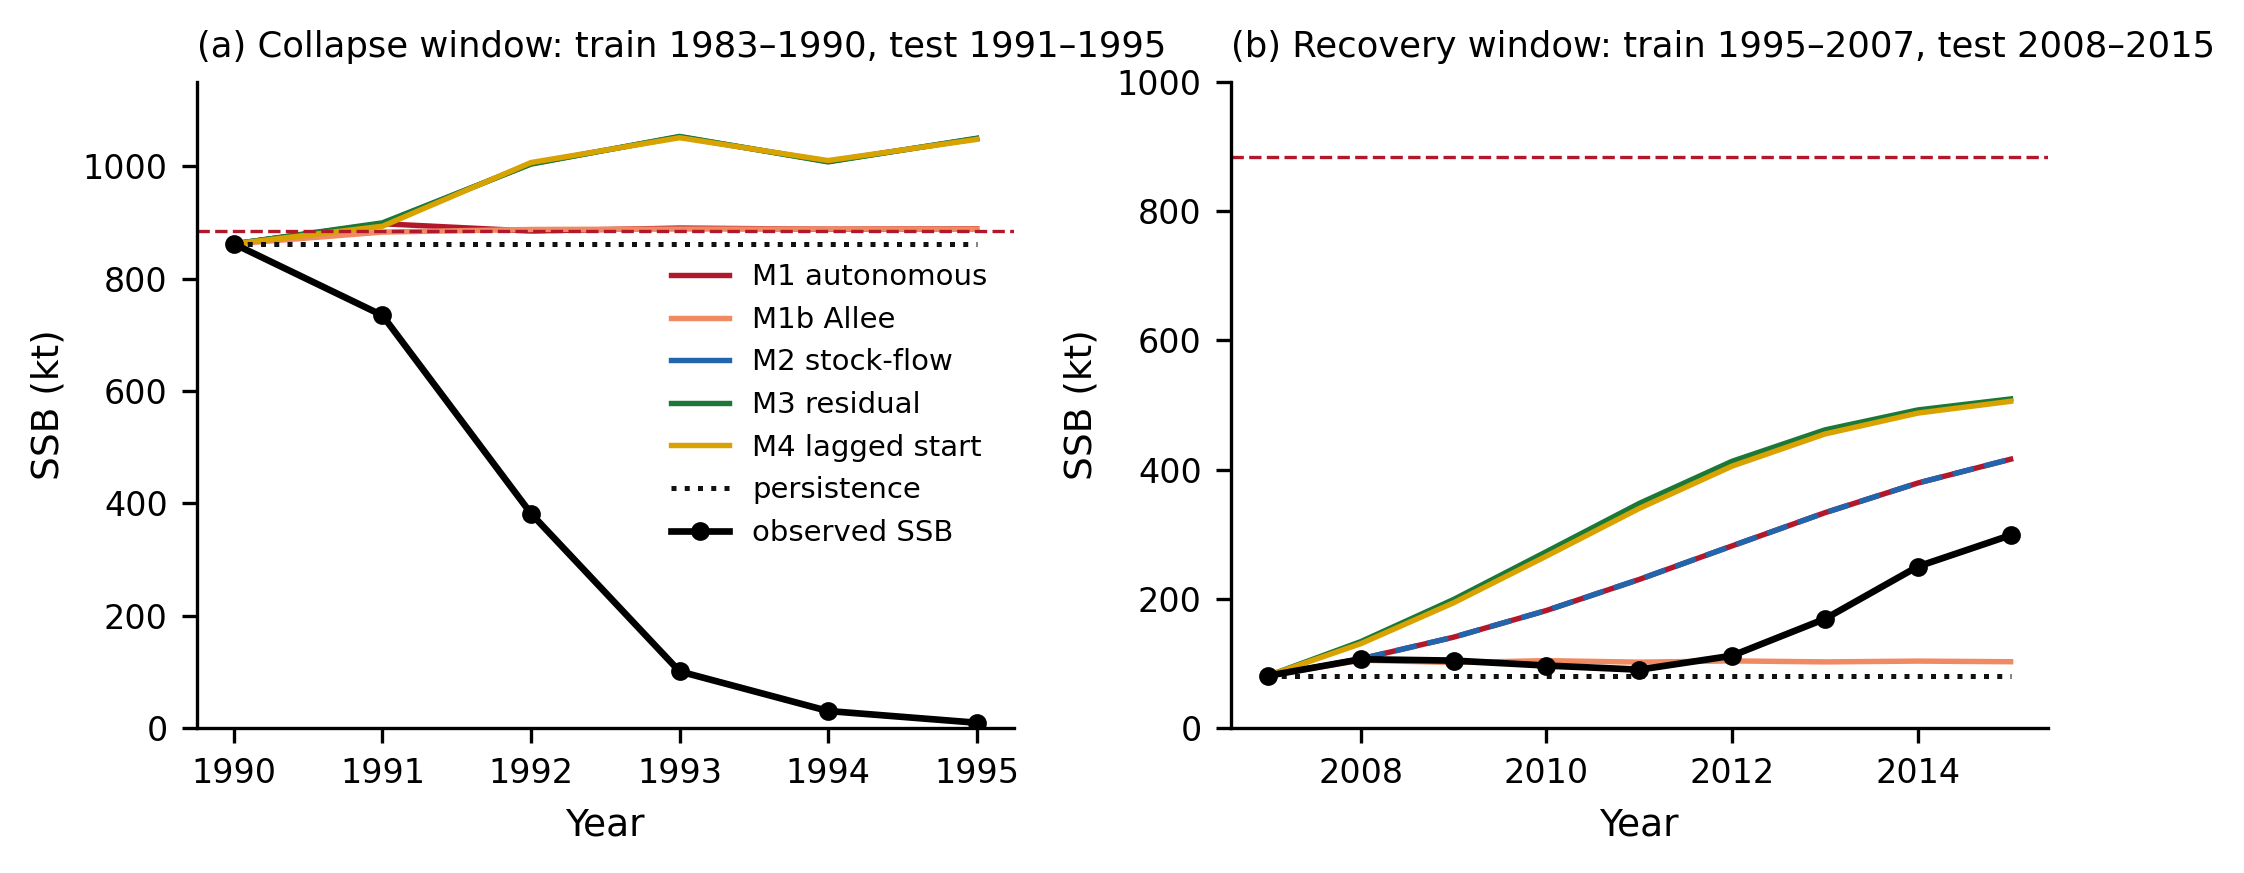
\includegraphics[width=\textwidth]{fig3_windows}
\caption{Fixed-window forecast paths on Specification A with the coarse-regime catch (the pass to which Table~\ref{tab:si_fixed} refers). (a) Collapse window: every module forecasts continuation or growth from the 1990 state; M1b lies under M1. (b) Recovery window: M1 and M2 coincide (training-mean and realised catch are both close to 5\,kt), M1b is a flat line at its fitted $K$, and M3 and M4 over-predict most because the last training residual, $+28\kt$ in 2006--2007, is carried forward with $\phi = 0.95$.}
\label{fig:si_windows}
\end{figure}

\FloatBarrier
\subsection*{S4.2 Variant passes}

Four variant passes were added after the primary pass and declared in order (S1), each scored against persistence recomputed on its own origin set (Table~\ref{tab:si_variants}). Replacing the coarse catch regime by annual landings on Specification A leaves the ordering unchanged. Starting the stock-flow forecast from a survey-scaled index value instead of the assessed state gives 128.1 and 331.0\,kt. Allowing the intrinsic rate to differ before and after the 1991 capelin collapse, the mechanism most often proposed for the post-collapse productivity regime, gives 153.8 and 334.0\,kt on A and 146.8 and 894.4 on B. Multiplying production by a capelin acoustic-index factor, which restricts the origins to the years with an acoustic estimate, gives 150.0 and 262.3\,kt on A against 96.6 and 193.0 for persistence on the reduced set, and 132.0 and 491.7 on B against 78.6 and 287.9. No variant comes within the band on either horizon.

\begin{table}[!htb]
\centering\footnotesize\setlength{\tabcolsep}{3.5pt}
\caption{Variant passes: rolling-origin RMSE (kt) of the variant module against persistence recomputed on the variant's origin set. $n$ is the number of origins at $h=1$ / $h=5$.}
\label{tab:si_variants}
\begin{tabular}{@{}llrrrr@{}}
\toprule
 & & \multicolumn{2}{c}{$h=1$} & \multicolumn{2}{c}{$h=5$} \\
Variant & Spec.\ ($n$) & module & persist & module & persist \\
\midrule
Annual landings, M2 & A (25/21) & 160.4 & 98.0 & 393.8 & 264.7 \\
Annual landings, M3 & A (25/21) & 153.6 & 98.0 & 351.5 & 264.7 \\
Annual landings, M4 & A (25/21) & 206.3 & 98.0 & 486.4 & 264.7 \\
Survey-start M2 & A (25/21) & 128.1 & 98.0 & 331.0 & 264.7 \\
Two-regime $r$ (1991 break) & A (25/21) & 153.8 & 98.0 & 334.0 & 264.7 \\
Two-regime $r$ (1991 break) & B (59/55) & 146.8 & 84.4 & 894.4 & 300.0 \\
Capelin-index multiplier & A (24/20) & 150.0 & 96.6 & 262.3 & 193.0 \\
Capelin-index multiplier & B (36/32) & 132.0 & 78.6 & 491.7 & 287.9 \\
\bottomrule
\end{tabular}
\end{table}
\FloatBarrier
\section{Fitted parameters}\label{si:params}

\begin{table}[!htb]
\centering\footnotesize\setlength{\tabcolsep}{3.5pt}
\caption{Fixed-window fits (one-step least squares on the training window). $\phi$ is the lag-one coefficient of the training residuals, clipped to $[-0.95,0.95]$; $\sigma$ their standard deviation (kt). M2--M4 share the stock-flow fit; M1 uses the training-mean catch, M1b the depensatory branch. Bounds: $r\in[10^{-3},2]$, $K\in[\max S+10,\,5000]$, $\sA\in[0,\max S]$; initialiser $r_0=0.3$, $K_0=\max(1.5\max S, 500)$.}
\label{tab:si_fixedfits}
\begin{tabular}{@{}llrrrrr@{}}
\toprule
Window (catch) & Module & $r$ & $K$ (kt) & $\sA$ (kt) & $\phi$ & $\sigma$ \\
\midrule
A collapse, train 1983--90 (coarse) & M1 & 1.935 & 1032.7 & -- & $-0.14$ & 33.8 \\
 & M1b & 2.000 & 1058.9 & 0.0 & $-0.65$ & 40.2 \\
 & M2--M4 & 1.935 & 1032.7 & -- & $-0.14$ & 33.8 \\
A recovery, train 1995--2007 (coarse) & M1 & 0.458 & 500.0 & -- & $0.95$ & 11.8 \\
 & M1b & 2.000 & 105.9 & 0.0 & $0.95$ & 11.7 \\
 & M2--M4 & 0.458 & 500.0 & -- & $0.95$ & 11.8 \\
A collapse (annual landings) & M1 & 1.942 & 1034.3 & -- & $-0.14$ & 33.8 \\
 & M1b & 2.000 & 1062.0 & 0.0 & $-0.66$ & 40.5 \\
 & M2--M4 & 1.991 & 1032.3 & -- & $-0.02$ & 47.0 \\
A recovery (annual landings) & M1 & 0.370 & 5000.0 & -- & $0.95$ & 11.8 \\
 & M1b & 2.000 & 129.8 & 0.0 & $0.95$ & 11.6 \\
 & M2--M4 & 0.390 & 5000.0 & -- & $0.95$ & 10.6 \\
\bottomrule
\end{tabular}
\end{table}

The $K$ estimate of the coarse-regime recovery fit, 500.0, is the initialiser $K_0 = \max(1.5\max S, 500)$: the objective is flat in $K$ above the observed range and the single L-BFGS-B start does not move it. Under annual landings the same fit runs to the 5000-kt upper bound. In both cases the production curve over the observed range (10--81\,kt) is effectively linear with slope $r$ (main-text Fig.~4).

\begin{table}[!htb]
\centering\scriptsize
\setlength{\tabcolsep}{4pt}
\caption{Specification A, coarse regime: parameters refitted at every rolling origin (expanding window from 1983). $\bar C$ is the training-mean catch used by M1 and M1b. From the 1992 origin, once the collapse transitions enter the training window, $K$ sits at its bound for the stock-flow fit and the depensatory threshold moves to 585--734\,kt; from 2011 it falls to about 5\,kt.}
\label{tab:si_rollingA}
\begin{tabular}{@{}lrrrrrrrrr@{}}
\toprule
 & \multicolumn{3}{c}{M2--M4 (stock-flow)} & \multicolumn{3}{c}{M1 (autonomous)} & \multicolumn{3}{c}{M1b (depensatory)} \\
\cmidrule(lr){2-4}\cmidrule(lr){5-7}\cmidrule(lr){8-10}
Origin & $r$ & $K$ & $\phi$ & $\bar C$ & $r$ & $K$ & $r$ & $K$ & $\sA$ \\
\midrule
1990 & 1.935 & 1033 & -0.14 & 240.0 & 1.935 & 1033 & 2.00 & 1059 & 0.0 \\
1991 & 1.557 & 1058 & -0.03 & 240.0 & 1.557 & 1058 & 2.00 & 1042 & 0.0 \\
1992 & 0.269 & 5000 & +0.34 & 228.0 & 0.252 & 5000 & 2.00 & 1192 & 672.7 \\
1993 & 0.250 & 5000 & +0.67 & 207.7 & 0.212 & 5000 & 2.00 & 2110 & 635.0 \\
1994 & 0.248 & 5000 & +0.57 & 190.8 & 0.190 & 5000 & 2.00 & 3049 & 585.3 \\
1995 & 0.248 & 5000 & +0.56 & 176.5 & 0.170 & 5000 & 2.00 & 3300 & 597.9 \\
1996 & 0.248 & 5000 & +0.56 & 164.3 & 0.153 & 5000 & 2.00 & 3271 & 628.8 \\
1997 & 0.248 & 5000 & +0.56 & 153.7 & 0.138 & 5000 & 2.00 & 3332 & 649.2 \\
1998 & 0.248 & 5000 & +0.56 & 144.4 & 0.125 & 5000 & 2.00 & 3453 & 663.6 \\
1999 & 0.248 & 5000 & +0.56 & 136.2 & 0.114 & 5000 & 2.00 & 3633 & 673.3 \\
2000 & 0.248 & 5000 & +0.56 & 128.9 & 0.104 & 5000 & 2.00 & 3942 & 676.1 \\
2001 & 0.248 & 5000 & +0.56 & 122.4 & 0.095 & 5000 & 2.00 & 4198 & 681.7 \\
2002 & 0.304 & 2537 & +0.58 & 116.5 & 0.087 & 5000 & 2.00 & 4373 & 690.6 \\
2003 & 0.247 & 5000 & +0.56 & 111.2 & 0.080 & 5000 & 2.00 & 4476 & 701.6 \\
2004 & 0.247 & 5000 & +0.56 & 106.4 & 0.073 & 5000 & 2.00 & 4547 & 713.0 \\
2005 & 0.247 & 5000 & +0.56 & 102.0 & 0.067 & 5000 & 2.00 & 4606 & 723.7 \\
2006 & 0.248 & 5000 & +0.56 & 97.9 & 0.061 & 5000 & 2.00 & 4768 & 730.7 \\
2007 & 0.248 & 5000 & +0.56 & 94.2 & 0.057 & 5000 & 2.00 & 5000 & 734.1 \\
2008 & 0.248 & 5000 & +0.56 & 90.8 & 0.054 & 5000 & 1.57 & 5000 & 707.8 \\
2009 & 0.248 & 5000 & +0.56 & 87.6 & 0.050 & 5000 & 1.12 & 5000 & 656.9 \\
2010 & 0.247 & 5000 & +0.56 & 84.6 & 0.047 & 5000 & 0.80 & 5000 & 588.7 \\
2011 & 0.246 & 5000 & +0.56 & 81.9 & 0.044 & 5000 & 0.13 & 1411 & 5.3 \\
2012 & 0.247 & 5000 & +0.56 & 79.3 & 0.042 & 5000 & 0.12 & 1411 & 5.3 \\
2013 & 0.247 & 5000 & +0.56 & 76.9 & 0.083 & 1408 & 0.11 & 1411 & 5.2 \\
2014 & 0.249 & 5000 & +0.56 & 74.7 & 0.148 & 1114 & 0.11 & 1411 & 5.1 \\
\bottomrule
\end{tabular}
\end{table}

\begin{table}[!htb]
\centering\scriptsize
\setlength{\tabcolsep}{4pt}
\caption{Specification B: range of the refitted parameters over the origins of each band. The depensatory threshold stays at or near zero throughout; the stock-flow $K$ is at or near its bound after 1993.}
\label{tab:si_rollingB}
\scriptsize\setlength{\tabcolsep}{2.5pt}
\resizebox{\textwidth}{!}{%
\begin{tabular}{@{}lrrrrrrrrr@{}}
\toprule
 & & \multicolumn{2}{c}{M2--M4} & \multicolumn{3}{c}{M1} & \multicolumn{3}{c}{M1b} \\
\cmidrule(lr){3-4}\cmidrule(lr){5-7}\cmidrule(lr){8-10}
Origins & $n$ & $r$ & $K$ & $\bar C$ & $r$ & $K$ & $r$ & $K$ & $\sA$ \\
\midrule
1965--1990 & 26 & 0.46--0.78 & 2482--5000 & 354--468 & 0.77--0.95 & 1845--2276 & 1.41--2.00 & 1642--2279 & 0.00--0.27 \\
1991--1995 & 5 & 0.50--0.59 & 3355--4800 & 317--349 & 0.71--0.83 & 1869--1922 & 1.57--1.76 & 1654--1660 & 0.00--0.00 \\
1996--2012 & 17 & 0.50--0.50 & 4802--5000 & 227--310 & 0.56--0.70 & 1789--1905 & 0.91--1.53 & 1651--2261 & 0.00--0.04 \\
2013--2023 & 11 & 0.47--0.50 & 5000--5000 & 193--223 & 0.53--0.57 & 1682--1774 & 0.81--1.09 & 1603--2261 & 0.00--0.04 \\
\bottomrule
\end{tabular}}

\end{table}

\begin{remark}[The compensatory branch is not the $\sA\to 0$ limit of the depensatory one]
Substituting $\sA = 0$ in $a(S) = (S-\sA)/(K-\sA)$ gives $a(S) = S/K$, so $g(S) = rS(1-S/K)(S/K)$, a cubic surplus, not the Schaefer form $a\equiv 1$. M1b at $\sA = 0$ is therefore a different model from M1, which is why the two differ slightly in the collapse window (693.6 against 694.3\,kt) even though both thresholds are at zero; what M1b adds to M1 is a branch of the family, not a limiting case of it.
\end{remark}

\begin{figure}[!htb]
\centering
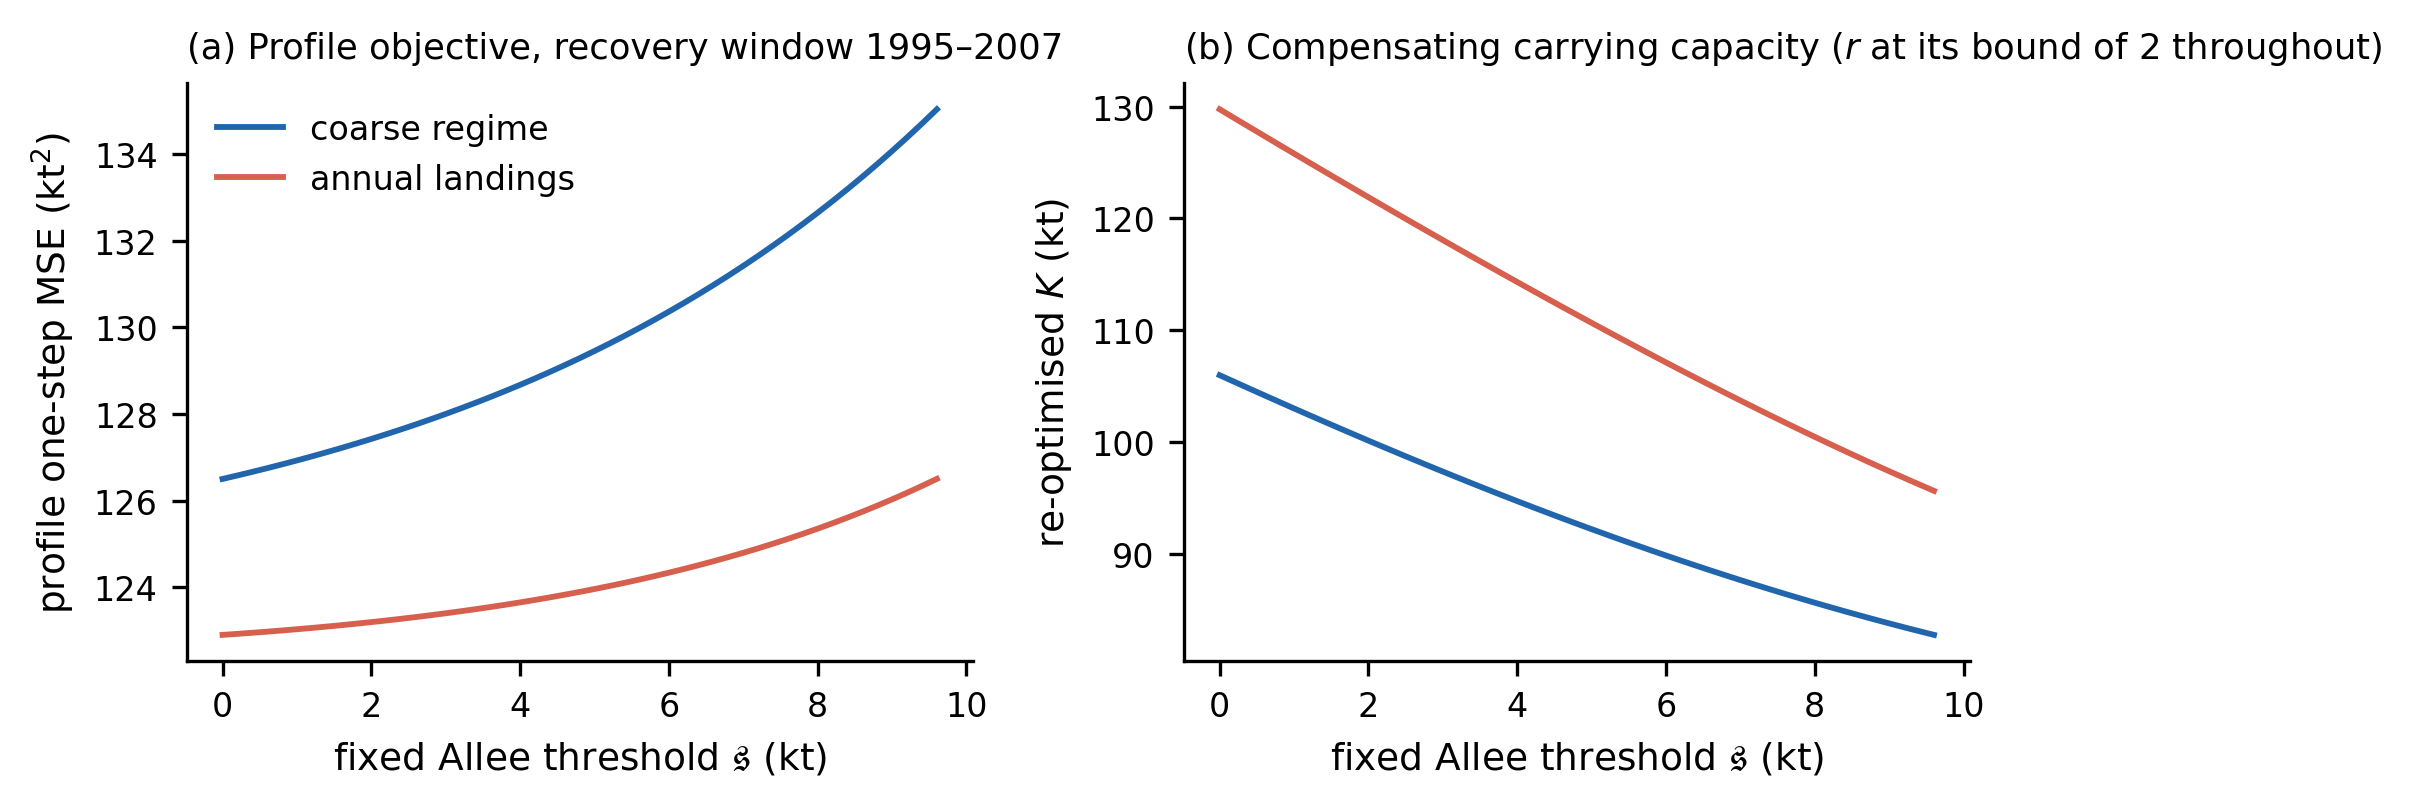
\includegraphics[width=\textwidth]{figS1_allee_profile}
\caption{Profile of the one-step objective over a fixed depensation threshold $\sA$ in the recovery window (train 1995--2007), with $r$ and $K$ re-optimised at each value. (a) The objective rises monotonically from $\sA = 0$ and changes by 6.7\% (coarse regime, 126.5 to 135.0\,kt$^2$) and 2.9\% (annual landings, 122.9 to 126.5) across the range below the smallest observed state (9.7\,kt). (b) The compensating $K$ falls as $\sA$ rises, with $r$ at its bound of 2 throughout. The threshold is unidentified in this window; its least-squares value is the boundary.}
\label{fig:si_profile}
\end{figure}

\FloatBarrier
\section{Floor-forecast census}\label{si:floor}

A forecast is at the floor when the iterated map reaches the numerical floor $\epsilon = 10^{-3}\kt$; its absolute error then equals the observed SSB. Table~\ref{tab:si_floor} counts floor forecasts by band from the archived per-origin files (coarse regime for Specification A). The counts in the first block are those behind the superscripts of Table 6 and Table~\ref{tab:si_h5}.

\begin{table}[!htb]
\centering\footnotesize\setlength{\tabcolsep}{3.5pt}
\caption{Number of origins at which the forecast is at the floor, by band and horizon.}
\label{tab:si_floor}
\begin{tabular}{@{}llrrrrrr@{}}
\toprule
Spec. & Origins & $n$ & M1 & M1b & M2 & M3 & M4 \\
\midrule
A, $h=1$ & 1990--1995 & 6 & 3 & 4 & 0 & 3 & 0 \\
A, $h=1$ & 1996--2012 & 17 & 12 & 13 & 0 & 0 & 0 \\
A, $h=1$ & 2013--2014 & 2 & 0 & 0 & 0 & 0 & 0 \\
A, $h=5$ & 1990--1995 & 6 & 4 & 4 & 1 & 3 & 1 \\
A, $h=5$ & 1996--2010 & 15 & 15 & 15 & 0 & 0 & 0 \\
B, $h=1$ & 1965--1990 & 26 & 2 & 3 & 0 & 0 & 0 \\
B, $h=1$ & 1991--1995 & 5 & 3 & 3 & 0 & 3 & 1 \\
B, $h=1$ & 1996--2012 & 17 & 17 & 17 & 0 & 0 & 0 \\
B, $h=1$ & 2013--2023 & 11 & 0 & 1 & 0 & 0 & 0 \\
B, $h=5$ & 1965--1990 & 26 & 10 & 17 & 7 & 7 & 7 \\
B, $h=5$ & 1991--1995 & 5 & 4 & 5 & 0 & 4 & 3 \\
B, $h=5$ & 1996--2012 & 17 & 17 & 17 & 0 & 0 & 0 \\
B, $h=5$ & 2013--2019 & 7 & 5 & 7 & 0 & 0 & 0 \\
\bottomrule
\end{tabular}
\end{table}

On Specification A the one-step M1 forecast is at the floor at every origin from 1993 to 2007; at 2008--2012 it forecasts 13--37\,kt from states of 91--169\,kt, and at 2013--2014 it forecasts 105 and 204\,kt against 250 and 299. The mechanism is the constant catch: at the 2000 origin the training-mean catch is 129\,kt (coarse) or 122\,kt (annual) against a state of 34\,kt, and at the 2010 origin 85 or 79\,kt against 91\,kt. On Specification B the training-mean catch is 317\,kt at the 1995 origin and still 201\,kt at the 2020 origin.

The log-RMSE diagnostic of the archived summaries uses $\log\max(\hat S,\epsilon)$ and is dominated by these floor forecasts; over the whole origin sets the floor binds for M1 at 15 of 25 ($h=1$) and 19 of 21 ($h=5$) origins on the Specification A annual pass and at 22 of 59 and 36 of 55 on Specification B, for M1b at 17/25, 19/21, 24/59 and 46/55, and for M2--M4 at between zero and eleven origins per cell. The raw RMSE, not the log column, is the retention score.

\FloatBarrier
\section{Secondary scores}\label{si:secondary}

\begin{table}[!htb]
\centering\footnotesize\setlength{\tabcolsep}{3.5pt}
\caption{Brier score of the hard below-threshold indicator implied by the point forecast ($\hat S < $ threshold against $S <$ threshold), origin-matched. Specification A uses the LRP of 884.6\,kt, below which every origin and target after 1990 lies, so the indicator never varies and persistence scores zero trivially; Specification B uses $\Blim = 276\kt$, which the series crosses in 1977, 1980, 1993 and 2016.}
\label{tab:si_brier}
\begin{tabular}{@{}lrrrr@{}}
\toprule
 & A, $h=1$ & A, $h=5$ & B, $h=1$ & B, $h=5$ \\
\midrule
persistence & 0.000 & 0.000 & 0.068 & 0.291 \\
M1 & 0.040 & 0.048 & 0.051 & 0.455 \\
M1b & 0.000 & 0.048 & 0.153 & 0.473 \\
M2 & 0.080 & 0.143 & 0.068 & 0.364 \\
M3 & 0.080 & 0.095 & 0.017 & 0.309 \\
M4 & 0.080 & 0.143 & 0.068 & 0.382 \\
\bottomrule
\end{tabular}
\end{table}

On Specification B the M3 indicator has the lowest one-step Brier score (0.017 against 0.068 for persistence: one misclassified crossing instead of four), and M1's five-year score (0.455) is the worst because it forecasts the floor through two decades in which the stock sat just below $\Blim$ and then crossed it. The direction-of-change score, the fraction of consecutive targets whose observed and forecast changes agree in sign, is 0.80--1.00 for the structural modules on Specification A and undefined for persistence (its forecast change is zero); it separates modules on an outcome that scarcely varies and carries no retention weight.

An interval-scale comparison is available on Specification B because the assessment publishes 95\% limits for its own predictand, with median relative width 0.44. Writing $D = |\hat S_{t+h|t} - S_{t+h}| / [(\mathrm{hi}_{t+h}-\mathrm{lo}_{t+h})/2]$, the proportion of hindcast errors not exceeding half the published width is 56\% for persistence, 36\% for M1 and 59\% for M3 at $h=1$ ($n=59$), and 18\%, 5\% and 7\% at $h=5$ ($n=55$). These are not coverage probabilities: the published interval expresses uncertainty about true biomass given the assessment's data, re-centring its width on a hindcast gives an interval with no established coverage, and the limits are right-skewed on the biomass scale (67 of 71 years asymmetric by more than 10\%). The statistic indicates only that hindcast discrepancies are of the same order as, or larger than, reported target-state uncertainty, and that M3 reads marginally above persistence on it at one step where the RMSE ordering does not.

\FloatBarrier
\section{Simulation: design and full decomposition}\label{si:sim}

\begin{table}[!htb]
\centering\footnotesize\setlength{\tabcolsep}{3.5pt}
\caption{Data-generating processes. All series have $T=33$ years (the Specification A length) with Gaussian process noise $\sigma\in\{11.8, 33.8\}\kt$ entering the state update; parameters are the archived fixed-window fits. Rolling origins use the eight-year minimum training length of Specification A. M3 and M4 were not simulated as truths.}
\label{tab:si_dgp}
\begin{tabularx}{\textwidth}{@{}lLL@{}}
\toprule
DGP & Generating process & Source of parameters \\
\midrule
D1 & M1 autonomous Schaefer, $r=1.935$, $K=1032.7$, $C\equiv 240$, $S_0 = 900$ & collapse-window coarse fit \\
D2 & M1 autonomous Schaefer, $r=0.458$, $K=500$, $C\equiv 5$, $S_0 = 30$ & recovery-window coarse fit \\
D3 & M2 stock-flow, $r=1.935$, $K=1032.7$, catch 240/120/5 along the Specification A schedule, $S_0=900$ & collapse fit and regime path \\
D4 & M1b depensatory, $r=0.458$, $K=500$, $\sA=15$, $C\equiv 5$, $S_0=30$ & recovery fit with an identifiable threshold \\
D5 & Persistence-true null, $S_{t+1} = S_t + \eta_t$, no production, $C\equiv 0$, $S_0=300$ & -- \\
D6 & Drifting productivity, $r_t = 1.935\,e^{-0.05t} + 0.35$, $K=1032.7$, catch 55\% of the instantaneous $r_tK/4$ & Amendment 1 (outside the class) \\
D7 & Smooth path: noise-free state at $r=0.9$, $K=1032.7$, $C=180$, scored series $=$ state plus Gaussian noise & Amendment 1 (outside the class) \\
\bottomrule
\end{tabularx}
\end{table}

The design sheet (\texttt{SPECIFICATION\_v4.md}) was locked at commit \texttt{d5d9758} on 2026-09-10 and the simulation code was written afterwards to implement it; no design element was changed after execution. Amendment 1 (D6, D7, and a $T=71$ series-length cell for D1 and D5) was locked at commit \texttt{bd0008f} on 2026-09-11; the $T=71$ cell was started and abandoned as infeasible (45.6\,s per rolling pass against 7\,s at $T=33$), so no series-length sensitivity is claimed. A module counts as retained in a replicate if it passes (H1)--(H3) at both horizons exactly as in the empirical rule.

\begin{table}[!htb]
\centering\footnotesize\setlength{\tabcolsep}{3.5pt}
\caption{Where the power is lost (averaged over the two noise levels). ``H2 alone'' is the persistence hurdle with the band at both horizons, ignoring the comparator.}
\label{tab:si_power}
\scriptsize\setlength{\tabcolsep}{2.5pt}
\begin{tabular}{@{}llrrrr@{}}
\toprule
DGP & truth & passes H2 alone & passes full rule & removed by comparator & conditional on H2 \\
\midrule
D1 & M1 & 0.975 & 0.975 & 0.000 & 0\% \\
D2 & M1 & 0.420 & 0.420 & 0.000 & 0\% \\
D3 & M2 & 0.328 & 0.100 & 0.228 & 69\% \\
D4 & M1b & 0.180 & 0.010 & 0.170 & 94\% \\
\bottomrule
\end{tabular}
\end{table}

\begin{table}[!htb]
\centering\footnotesize\setlength{\tabcolsep}{3.5pt}
\caption{Chance baseline: proportion of replicates in which the generating module has the lowest one-step RMSE among the five modules (chance $=0.20$).}
\label{tab:si_chance}
\begin{tabular}{@{}lrl@{}}
\toprule
DGP & true module ranks first & against chance \\
\midrule
D1 (M1 true) & 0.627 & far better \\
D2 (M1 true) & 0.645 & far better \\
D3 (M2 true) & 0.038 & worse than chance \\
D4 (M1b true) & 0.258 & barely better \\
\bottomrule
\end{tabular}
\end{table}

In absolute terms the dominant failure is the persistence hurdle: a true module often does not out-predict persistence on data it generated. Conditional on clearing it, the comparator hurdle removes most of the survivors for the stock-flow and depensatory truths. On D3 the stock-flow module's mean one-step error (85.7\,kt) exceeds that of the residual (77.9) and depensatory (79.9) modules, so estimation noise actively disadvantages the correct structure relative to its siblings at this sample size. Under the four structural processes the false-retention rate is 0.044 per module--replicate pair (0.176 falsely retained modules per replicate); under the persistence-true null it is 0.005 per module. Under D6 and D7 the module falsely retained is overwhelmingly M1 (134 and 151 of 200 replicates under D6, 195 and 185 under D7): a constant-productivity map out-predicts persistence on a smoothly drifting or smoothly observed series often enough to clear both hurdles. The alternative decision rules of Table 8 were evaluated on the same archived replicates without refitting.

Two candidate diagnostics for predicting from the data alone whether the rule has power were examined and both fail. The dispersion of scores across modules (median coefficient of variation) correlates with true-module power at Spearman $\rho = 0.52$, too weakly to license a protocol. The margin of the best-scoring module over persistence correlates at $\rho = 0.88$ (Pearson $r = 0.94$) but is computed from the same out-of-sample scores the rule consumes, so it cannot gate the decision, and thresholding it at the tie band misclassifies both D3 cells, flagging ``apply'' where the generating module wins less often than chance. Identifying when the rule has power remains open.

\FloatBarrier

\begin{table}[!htb]
\centering\footnotesize\setlength{\tabcolsep}{3.5pt}
\caption{Alternative decision rules evaluated on the archived simulation replicates. Mean power is averaged over D1--D4 and both noise levels; specificity is one minus the false-retention rate under D5, both noise levels. In-class truths only; under D6--D7 no rule examined is specific.}
\label{tab:si_rules}
\begin{tabular}{@{}lrr@{}}
\toprule
Decision rule & mean power & specificity \\
\midrule
Protocol C as adopted (C1--C3, 5\% band) & 0.376 & 0.978 \\
Without the comparator hurdle (C2, C3 only) & 0.476 & 0.972 \\
Persistence only, $h=1$, 5\% band & 0.562 & 0.955 \\
Persistence only, any margin & 0.542 & 0.765 \\
Full rule, no tie band & 0.436 & 0.772 \\
Full rule, 10\% band & 0.337 & 0.998 \\
MASE $<1$ against the naive benchmark & 0.651 & 0.675 \\
Information criterion, $n\log\mathrm{MSE} + 2k$ & 0.509 & 0.992 \\
\bottomrule
\end{tabular}
\end{table}

\section{Decomposition of the lagged-start deficit}\label{si:m4}

M4 differs from M3 in two ways: it starts the path from $S_{t-1}$, and it therefore integrates one more catch year. A delayed-persistence control, $\hat S_{t+h} = S_{t-1}$, isolates the information delay. Its one-step RMSE is 184.4\,kt on Specification A and 158.0\,kt on Specification B, against 98.0 and 84.4 for ordinary persistence; the delay alone therefore costs 86.4 of M4's 97.5-kt deficit against persistence on A and 73.6 of 121.3 on B. The lagged start is an information-delay penalty, not a dynamical one, and M4 is not retained for the same reason that a one-year-stale persistence forecast would not be.

\FloatBarrier
\section{The outcome years 2016--2021}\label{si:outcome}

Specification A ends in 2015. The continuation of the same assessment family is published in the RAM Legacy Stock Assessment Database (v4.66, stock COD2J3KL), and xteNCAM reads the same years independently (Table~\ref{tab:si_outcome}). Every year 2016--2021 lies above its 2015 origin in both vintages, so the window contains no event of the kind the collapse test probes, and persistence from the 2015 origin errs low throughout: MAE 129.2\,kt and RMSE 133.3\,kt on the RAM vintage (107.5\,kt MAE from the Table A2 origin of 298.65\,kt), the same order as its scored one-step RMSE. The two vintages agree on the outcome years to within 1--26\,kt (mean 16.8), while on the historical overlap they do not (S11). The restatement of the Edwards J-17 scores under Protocol C, which the single-system edition carried here, is now in main-text Section 4.3.

\begin{table}[!htb]
\centering\footnotesize\setlength{\tabcolsep}{3.5pt}
\caption{Outcome years on the Specification A horizon. Persistence error is $|S_t - S_{2015}|$ from the RAM-vintage 2015 origin of 277\,kt; the xteNCAM column is the revised model's reading of the same years.}
\label{tab:si_outcome}
\begin{tabular}{@{}lrrrr@{}}
\toprule
Year & RAM v4.66 (kt) & xteNCAM (kt) & $|$difference$|$ & persistence error (kt) \\
\midrule
2016 & 340 & 339 & 1 & 63 \\
2017 & 433 & 451 & 18 & 156 \\
2018 & 394 & 369 & 25 & 117 \\
2019 & 419 & 400 & 19 & 142 \\
2020 & 440 & 414 & 26 & 163 \\
2021 & 411 & 423 & 12 & 134 \\
\bottomrule
\end{tabular}
\end{table}
\FloatBarrier
\section{Vintages and thresholds}\label{si:thresholds}

\paragraph{Vintage overlap, 1983--2015} The NCAM Table A2 vintage (Specification A) and the RAM Legacy v4.66 continuation of the same assessment family (stock COD2J3KL) differ over 1983--2015 by $+24.7\kt$ on average (Table A2 higher), by 26.8\,kt in mean absolute value and by 131.2\,kt at most, in 1984 (Fig.~\ref{fig:si_vintages}). The xteNCAM revision differs from Table A2 over the same years by 126.2\,kt RMSE, with Table A2 higher by 58.5\,kt on average. The 2015 origin is 298.65\,kt on Table A2, 277\,kt on RAM and 273\,kt on xteNCAM.

\paragraph{Vintage-shifted LRP} The LRP defined as the 1983--1989 mean is 884.6\,kt on the Table A2 vintage and 790.0\,kt on the RAM vintage, a shift of 94.6\,kt in the reference point from a revision of the same model family. Persistence from the 2015 origin under-predicts every outcome year 2016--2021 in both vintages: MAE 129.2\,kt and RMSE 133.3\,kt from the RAM origin of 277\,kt, MAE 107.5\,kt from the Table A2 origin. The outcome years agree across the RAM and xteNCAM vintages to within 1--26\,kt (mean absolute difference 16.8\,kt).

\paragraph{Threshold classification on one file} The xteNCAM file (1954--2024, 71 years) carries a ratio column that fixes $\Blim$ at 276\,kt (per-year implied values 250--289, mean 275.5). Classifying each year under $\Blim = 276\kt$ and under the 884.6-kt LRP gives 45 years at or above $\Blim$, 16 years at or above the LRP (1954--1969 only), and 29 disagreement years in two blocks: 1970--1992 without 1977--1979, and every outcome year 2016--2024. Under the 1980s-mean threshold the stock stands below the reference point for 55 consecutive years (1970--2024); under $\Blim$ it is below for 26 years (1977--1979 and 1993--2015) and above from 2016 onward. The late-1970s episode (ratios 0.69--0.95) is a critical-zone reading, on the current model, of years the contemporary fishery regarded as healthy. The checkpoints 2005, 2017 and 2024 read 26, 451 and 342\,kt. The October 2023 framework revision, which moved the stock's reported zone from critical to cautious without a change in the stock, is this experiment executed by the assessment authority. The scored RMSE comparison never uses the thresholds; every normative verdict layered on the forecasts, the Brier indicator included, inherits the dependence.

\begin{figure}[!htb]
\centering
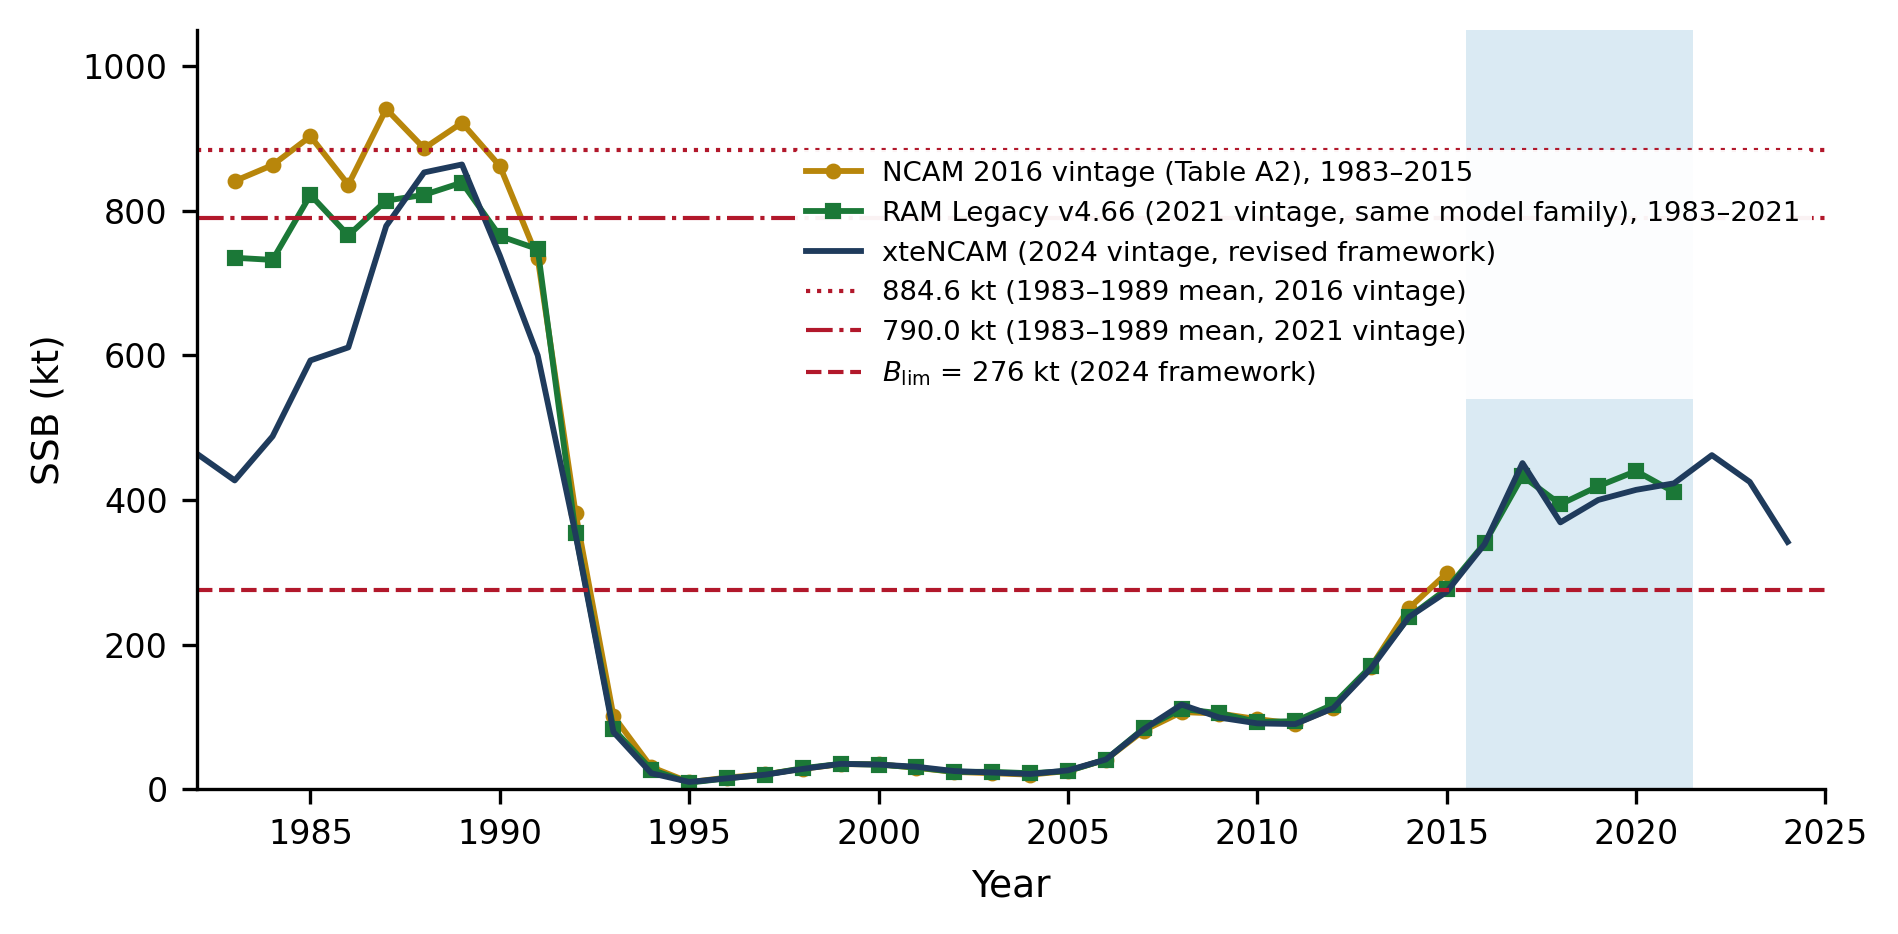
\includegraphics[width=\textwidth]{figS2_vintages}
\caption{Three vintages of Northern cod SSB over 1983--2024: NCAM Table A2 (Specification A, 1983--2015), RAM Legacy v4.66 (the same assessment family continued to 2021) and xteNCAM Table 17 (Specification B). Horizontal lines mark the two Specification A LRP values (884.6\,kt on Table A2, 790.0\,kt on the RAM vintage) and $\Blim = 276\kt$. The outcome years 2016--2021 lie above the 2015 origin in every vintage and below 884.6\,kt in every vintage.}
\label{fig:si_vintages}
\end{figure}

\FloatBarrier
\section{The 2022--2023 observation suspension}\label{si:suspension}

The test conditions on a complete annual series. The stock's real 2022--2023 history violates that condition. Partial coverage by the fall research-vessel survey in 2021 and 2022 left the leading indicator of stock size uncomputable; no typical assessment update was possible in 2022 or 2023; the stewardship maximum was rolled over unchanged at 12{,}999 t; and the survey vessel that carries the series was condemned in February 2023. Table~\ref{tab:si_suspension} assembles the episode from the assessment of record and the public record.

\begin{table}[!htb]
\centering\footnotesize\setlength{\tabcolsep}{3.5pt}
\caption{The 2022--2023 observation suspension and its resolution (sources: Regular et al.\ 2025 and its Table 17 file; the 2024 reopening announcement; the 2025 and 2026 assessment coverage).}
\label{tab:si_suspension}
\begin{tabularx}{\textwidth}{@{}lL@{}}
\toprule
Period & Event \\
\midrule
2021--22 & Partial fall-survey coverage; leading indicator not computable \\
2022--23 & No typical assessment update; stewardship maximum held at 12{,}999 t \\
Feb 2023 & Survey vessel condemned \\
Mar 2024 & Revised-framework assessment: SSB at 1.2 \(B_{\mathrm{lim}}\) (95\% CI 0.7--2.1; 22\% critical-zone probability) \\
Jun 2024 & Commercial fishery reopened at 18{,}000 t after 32 years \\
2025 & TAC 38{,}000 t; reference point revised after being deemed overestimated \\
Apr 2026 & Healthy-zone report: SSB $\approx$ 540 kt (CI 420--700); 70\% probability above the upper stock reference \\
\bottomrule
\end{tabularx}
\end{table}

Read against a review-timing rule under which a review must land no later than the worst-case loss of the information it consumes, the episode is that rule's boundary case in the wild: the information loss ran past the review cadence, and the removals rule froze for two cycles while the observation map was dark. Abaee (2026, Periodic review as sampled governance) states the formal identity; the 2022--2023 suspension is its empirical instance, and it marks the practical limit of any scoring exercise that presumes the series exists.

\FloatBarrier
\section{Reproducibility and verification record}\label{si:repro}

\paragraph{Determinism} All computations are deterministic: within a fixed interpreter and library stack, repeated executions reproduce every result file byte for byte. An independent re-execution verified all 29 recorded output checksums and regenerated all 30 result files byte-identically; one archived file carries no pinned checksum and is covered by the regeneration comparison. Across environments (Python 3.12, numpy 2.1.3, scipy 1.14.1 against the recorded original environment), the intervention runners and the OLS-based prediction runners regenerate their outputs byte for byte, while the four optimiser-based forecast runners (L-BFGS-B fits) reproduce every scored row at printed precision with one exception: the M1b rolling row on Specification B, whose depensatory optimum is environment-sensitive at the $\pm17\kt$ level ($h=1$: 151.6 against 153.2\,kt; $h=5$: 445.5 against 462.5\,kt). That sensitivity is the identification fragility of Section~\ref{si:params} and is immaterial to the verdict, which persistence wins at both horizons by margins far larger than the instability.

\paragraph{Third environment (preceding edition)} For the preceding single-system edition the four forecast runners (\texttt{run\_ladder.py}, \texttt{run\_xte.py}, \texttt{run\_capelin\_regime.py}, \texttt{run\_capelin\_index.py}), the uncertainty script and the simulation outputs were re-executed or re-read in a third environment (Python 3.13.16, numpy 2.3.5, scipy 1.17.1). Every result file, including the M1b rows, was reproduced at printed precision, and the persistence baselines were recomputed from the series on the archived origin sets and matched the archived origin-matched values (98.05, 264.72, 84.43, 299.98\,kt). The paired block bootstrap was re-run from the archived per-origin files with an explicitly shared index draw and reproduced every interval of Table~\ref{tab:si_dm}. The period decomposition, the rolling parameter record, the floor census and the catch-timing sensitivity were computed in the same environment from the archived files and the unmodified runner functions; their scripts are archived under \texttt{paperE1\_cod\_forecast\_ladder\_v69\_src/work/}. The present edition re-reads the archived result files and recomputes the two baselines on the archived origin sets (S23); no forecast runner was re-executed and no archived cod score changed.

\paragraph{Verification script} \texttt{paper11\_forecasting\_\allowbreak{}baselines\_v67\_\allowbreak{}verification.py} (standard library only) regenerates every number of main-text Section 3.7, of S10 and of Sections~\ref{si:thresholds}--\ref{si:suspension} from the archived data files (NCAM Table A2, RAM v4.66 time series, xteNCAM Table 17, the capelin index) and asserts the cross-checks, including the presence in the manuscript source of the pinned values and the suspension facts. All checks pass on the main text and this document taken together.

\paragraph{Scripts} (\texttt{SRC} denotes the source folder \texttt{paper11\_forecasting\_\allowbreak{}baselines\_v67\_src} of the repository.)
{\footnotesize\begin{verbatim}
python3 wave_e_cod/src/run_ladder.py
python3 wave_e_cod/src/run_xte.py
python3 wave_e_cod/src/run_capelin_regime.py
python3 wave_e_cod/src/run_capelin_index.py
python3 "campaign_e1_dm_uncertainty_regime.py"
python3 tools/sim_retention_power.py
python3 SRC/work/cod/paired_bootstrap.py
python3 SRC/work/cod/post1995.py
python3 SRC/work/cod/catch_timing_sensitivity.py
python3 SRC/work/cod/make_figures.py
\end{verbatim}}

\FloatBarrier
\section{Catch-timing convention: a sensitivity outside the archived protocol}\label{si:timing}

In \texttt{run\_ladder.py} the estimator pairs the increment $S_{j+1}-S_j$ with the catch $C_j$ of the same year, whereas the forecast path at origin $t$ applies $C_{t+1},\dots,C_{t+h}$ to the steps $t\to t+1,\dots,t+h-1\to t+h$. The two conventions differ by one year. The estimation convention is the one under which SSB is a start-of-year quantity and $C_t$ the removals during year $t$; the forecast convention gives the catch-supplied modules the catch of the target year, which under that reading occurs after the predictand is realised. The offset was noticed during the re-execution for this revision. Table~\ref{tab:si_timing} re-runs M2--M4 with the estimation convention in the forecast path (persistence and M1/M1b are unaffected). Under the coarse regime the two conventions differ only at the 1990--1992 origins, where the regime boundaries fall; under annual landings and on Specification B they differ at every origin.

\begin{table}[!htb]
\centering\footnotesize\setlength{\tabcolsep}{3.5pt}
\caption{Rolling-origin RMSE (kt) of the catch-supplied modules under the archived forecast convention ($C_{t+1}$ applied to the step $t\to t+1$) and under the estimation convention ($C_t$), with the ratio to origin-matched persistence in parentheses.}
\label{tab:si_timing}
\begin{tabular}{@{}llcrrr@{}}
\toprule
Spec.\ (catch) & Module & $h$ & archived & estimation convention & persistence \\
\midrule
A annual & M2 & 1 & 160.4 (1.64) & 133.3 (1.36) & 98.0 \\
A annual & M2 & 5 & 393.8 (1.49) & 390.8 (1.48) & 264.7 \\
A annual & M3 & 1 & 153.6 (1.57) & 125.5 (1.28) & 98.0 \\
A annual & M3 & 5 & 351.5 (1.33) & 352.2 (1.33) & 264.7 \\
A annual & M4 & 1 & 206.3 (2.10) & 161.9 (1.65) & 98.0 \\
A annual & M4 & 5 & 486.4 (1.84) & 438.7 (1.66) & 264.7 \\
A coarse & M2 & 1 & 144.1 (1.47) & 113.4 (1.16) & 98.0 \\
A coarse & M2 & 5 & 398.2 (1.50) & 367.8 (1.39) & 264.7 \\
A coarse & M3 & 1 & 134.6 (1.37) & 105.2 (1.07) & 98.0 \\
A coarse & M3 & 5 & 366.4 (1.38) & 341.5 (1.29) & 264.7 \\
A coarse & M4 & 1 & 195.6 (1.99) & 138.9 (1.42) & 98.0 \\
A coarse & M4 & 5 & 488.2 (1.84) & 409.8 (1.55) & 264.7 \\
B & M2 & 1 & 166.0 (1.97) & 146.4 (1.73) & 84.4 \\
B & M2 & 5 & 1058.9 (3.53) & 981.8 (3.27) & 300.0 \\
B & M3 & 1 & 126.7 (1.50) & 94.9 (1.12) & 84.4 \\
B & M3 & 5 & 930.1 (3.10) & 832.5 (2.78) & 300.0 \\
B & M4 & 1 & 205.7 (2.44) & 130.3 (1.54) & 84.4 \\
B & M4 & 5 & 1030.7 (3.44) & 898.3 (2.99) & 300.0 \\
\bottomrule
\end{tabular}
\end{table}

Under the estimation convention every one-step deficit shrinks and no five-year deficit changes sign. M3 is 7\% above persistence at one year on Specification A (coarse) and 12\% on Specification B, still outside the 5\% band, and 29\% and 178\% above at five years. The post-1995 bands of Table 6 are unchanged on Specification A (the catch is constant at 5\,kt there under the coarse regime); on Specification B the post-1995 one-step M3 margin becomes $+10.4\kt$ with interval $[-20.2, +46.8]$ ($p = 0.53$), M2 and M4 remain significantly worse ($+62.0$, $[+24.6, +98.7]$; $+45.9$, $[+11.8, +86.4]$), and all five-year margins remain far outside the band. The verdict of the main text does not depend on the convention; the size of the one-step deficits does, and a future application of the ladder should use the estimation convention throughout.

\begin{figure}[!htb]
\centering
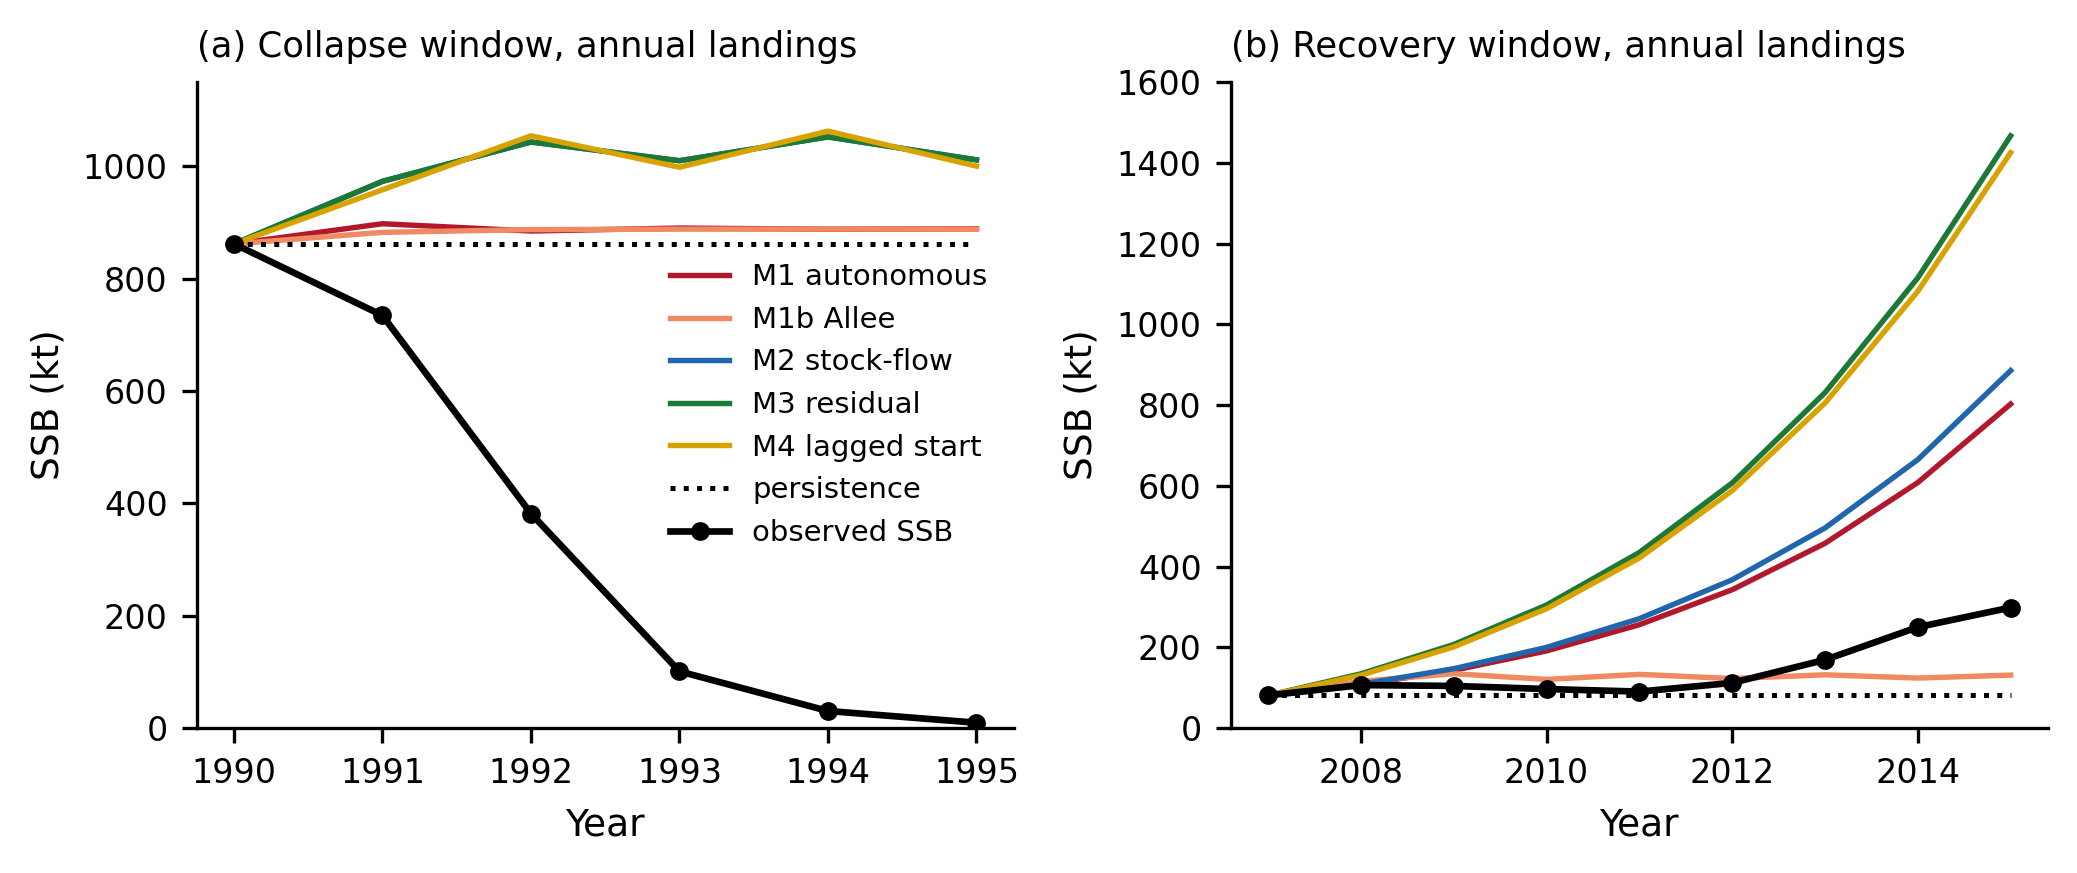
\includegraphics[width=\textwidth]{figS3_windows_annual}
\caption{Fixed-window forecast paths on Specification A with annual landings (companion to Fig.~\ref{fig:si_windows} in S4). (a) Collapse window: as under the coarse regime, every module forecasts continuation or growth. (b) Recovery window: with $K$ at its 5000-kt bound, production does not saturate and the catch-supplied modules over-predict more than under the coarse regime (M3 609\,kt RMSE against 220); M1b is again a flat line at its fitted $K$.}
\label{fig:si_windows_annual}
\label{fig:si_annual}
\end{figure}
\FloatBarrier
\part*{Part B: Edwards Aquifer, index well J-17}
\addcontentsline{toc}{part}{Part B: Edwards Aquifer}

\section{Protocol record and deviations}\label{si:edwprotocol}

The scoring protocols for the primary pass and the climate pass were frozen and dated (2026-08-25) before the corresponding RMSE tables were computed, and are archived with the analysis code. The design is a fixed computational protocol rather than a prospective registration; the phrase ``pre-registered'' is avoided for that reason. The retention rule as frozen reads, verbatim:

\begin{quote}\small
Let $\mathrm{RMSE}(\cdot)$ denote the primary rolling-origin RMSE at a fixed horizon $h$. A causal module $M$ is retained only if: (H1) $\mathrm{RMSE}(M) < \mathrm{RMSE}(\text{persist})$, i.e.\ it beats last-value persistence, and (H2) $\mathrm{RMSE}(M) < \mathrm{RMSE}(M_{\text{next-simpler causal}})$, i.e.\ it beats the next-simpler causal model. Retention is decided at $h=1$ on the point-RMSE comparison; no tie tolerance and no minimum margin is imposed. Diagnostic oracles are excluded from retention. The Comal series is excluded from retention. Retention is decided on the head series only; the service series is scored after that decision is frozen.
\end{quote}

The main text labels these hurdles (E1) and (E2). The primary score is RMSE of annual-mean J-17 in feet; secondary scores are mean absolute error and the Brier score of $\mathbf{1}\{\hat H<660\}$, interpreted only for origins at or after 2007 (S19). A sign-hit rate of $\Delta H$ was listed in an earlier design iteration and is struck: no value is reported for it and it is not part of any retention decision.

Three protocol elements sit outside the frozen rule and are recorded here as deviations, in one place.
\begin{enumerate}[leftmargin=2em]
\item \textbf{The M2m class clause.} M2m is listed and then declined on class grounds (main-text Remark~1). The clause is in the frozen protocol document, but it is not in the retention rule; under the rule as written, M2m satisfies (E1) and (E2) at $h=1$ (12.28 against 13.23 and 12.84\,ft).
\item \textbf{The climate-rung comparator.} The frozen Pass-2 protocol states the climate question as whether a causal recharge forecast reduces primary RMSE on J-17 ``relative to persistence and relative to M1'', the retained M1. The comparator is read accordingly. Declaring the declined M2m as the rung's (E2) comparator would be inconsistent with the frozen document and circular, since the gate would be a model the protocol had itself declined. The M2m margins are retained as a nested-baseline reading rather than as the gate. The choice changes no frozen verdict (no climate module is retained under either statement).
\item \textbf{The struck sign-hit score.}
\end{enumerate}

Post-freeze objects, labelled as such: the climate-pass fixed-window scores (S22), the pumpage counterfactuals (S21), the Comal service-series scoring (S20), and the uncertainty layer (S18) together with its independent replication. None replaces or alters a frozen verdict.

\section{Origin sets, windows and data processing}\label{si:edworigins}

\paragraph{Rolling origin} Minimum 15 training years; the first origin is 1948 and forecasts target years through 2023, giving $n=75$ origins at $h=1$ and $n=71$ at $h=5$. Every model in the rolling tables, including M2m and the climate variants, is scored on the identical origin sets. Early rolling origins with the 15-year floor give 14 transitions for a four-parameter fit, so the causal family's rolling scores carry unstable early-window coefficients.

\paragraph{Fixed windows} (1) Drought-of-record drawdown: train 1934--1950 (16 transitions), test 1951--1956. (2) Drought-of-record recovery: train 1934--1956 (22), test 1957--1961. (3) Pre-permit wet interval: train 1980--1990 (10), test 1991--1995. (4) Critical-period era: train 1997--2014 (17), test 2015--2023.

\paragraph{Head series} Annual means use all available daily highs of TWDB well 6837203. Years with fewer than 240 observations would be dropped; no year falls below the floor (minimum $n=242$, 1939), so the rule never binds. 1935 ($n=258$) and 1939 ($n=242$) are retained as incomplete-coverage means; missing days are not interpolated; the published pre-continuous composite (Beverly Lodges extension) is used as issued; the complete estimation panel ends in 2023, whose values carry provisional TWDB status. The predictand is the calendar-year mean of daily \emph{highs}; a daily-mean convention would sit slightly lower and matters near the 660/618-ft lines, and the Authority's Stage~I rule is a 10-day mean, so the annual-mean indicator is a coarse proxy flagged where used. Stage~I at 660\,ft is a 2007 institutional rule and is not applied as if it existed in 1956.

\paragraph{Fluxes and climate} Recharge $R$ is USGS total San Antonio-area recharge ($10^3$ acre-ft\,yr$^{-1}$), Puente stream-loss method, constructed independently of J-17 (Umphres and Choi, 2025). Pumpage $P$ is well discharge from Edwards Aquifer Authority Table~1 (1934 onward). Total spring discharge is stored and not used as a driver; eastern-basin recharge was stored and not used. Climate predictors: September--November Ni\~no~3.4 (HadISST, anomaly relative to 1991--2020) and calendar-year precipitation in Texas climate divisions 06 and 07 (NCEI nClimDiv). December--February precipitation that includes January of $t+1$ is not used. The registered twenty-column analysis panel (\texttt{wave\_e\_edwards/data/annual\_panel.csv}) is the dataset of record for all scored analyses; the nClimDiv raw file is not redistributed (provenance URL archived), so its three columns rebuild from the provenance source rather than from the archive, while the two Ni\~no columns rebuild from the registered file to machine precision.

\paragraph{Information set} Information known at 31 December of year $t$ comprises $(H,R,P)$ through $t$, the September--November Ni\~no~3.4 anomaly of year $t$ and calendar-year precipitation of year $t$. A two-pool exchange module was specified and not fitted; no barrier or exchange term was fitted. Post-1997 pumpage no longer spikes with drought as in 1956 ($321\times10^3$ acre-ft from wells); that change is already in $P_t$, and a separate critical-period switch adds no degree of freedom beyond the pumpage series.

\FloatBarrier
\section{Fixed windows}\label{si:edwfixed}

Table~\ref{tab:si_edwfixed} and Fig.~\ref{fig:si_edwwindows} give the fixed-window scores. They are diagnostic, not retention. On the drawdown window the bolded M2 is a continuing-drought artefact, not a forecasting merit: the last observed $R$ is already low, and the map trained on 1934--1950 has the wrong sign on pumpage ($\gamma=+0.021$), since pumping rose as the drought deepened and least squares aliases the human response into the state transition (simultaneity bias, compounded by the short window). That identification failure is why M2 ``beats'' the oracle there. The train-mean baseline is the best non-oracle forecast on the recovery window (14.07\,ft) and the critical-period era (14.77\,ft), consistent with its rolling five-year win; the residual-persistence rungs M3/M4 track M2 on the drawdown (18.12/18.23 against 18.11\,ft); M4 is the best causal model on the pre-permit wet window (15.26\,ft); and both fail with the causal family on the recovery and critical-period windows.

The recovery window is also where the $[610,710]$ clip binds on forecast paths: the M2 trajectory with persisted $(R,P)=(43.7,321.1)$ runs $617.1\to611.6\to606.8\to605.3\to605.3$\,ft, reaching the 610-ft floor from 1959 onward. The clip never binds on the observed record (annual means 623--692\,ft); it binds only on these persisted-drought forecast paths, and it is doing work exactly there. The audit script recomputes both fixed-window M2 RMSEs (18.11 and 55.32\,ft) exactly from the registered panel. The 1957--61 recovery is a recharge pulse ($R_{1956}=43.7$, $R_{1957}=1142.6\times10^3$ acre-ft): persistence stays at the 1956 floor, M2 persists drought recharge and falls further, the oracle, given the 1957 flood year, tracks the rise. Recoveries on this specification are recharge events, not autonomous mean reversion, although the training mean (mean reversion) scores 14.07\,ft, second only to the oracle, in this institutionally bounded, rapidly recharged system.

\begin{table}[!htb]
\centering\footnotesize\setlength{\tabcolsep}{3.5pt}
\caption{J-17 fixed-window RMSE (ft). Bold marks the lowest RMSE of the window including the diagnostic oracle.}
\label{tab:si_edwfixed}
\begin{tabular}{@{}lrrrrrrrr@{}}
\toprule
Window & persist & mean & M1 & M2 & M2m & M3 & M4 & oracle \\
\midrule
Drawdown 1951--56 & 23.75 & 35.19 & 30.94 & \textbf{18.11} & 27.44 & 18.12 & 18.23 & 19.69 \\
Recovery 1957--61 & 43.62 & 14.07 & 56.24 & 55.32 & 37.74 & 55.28 & 55.12 & \textbf{12.26} \\
Pre-permit wet 1991--95 & 30.13 & 18.24 & 20.02 & 16.67 & 23.47 & 16.41 & 15.26 & \textbf{7.18} \\
Critical-period era 2015--23 & 27.41 & 14.77 & 15.62 & 23.37 & 14.79 & 22.84 & 22.17 & \textbf{8.70} \\
\bottomrule
\end{tabular}
\end{table}

\begin{figure}[!htb]
\centering
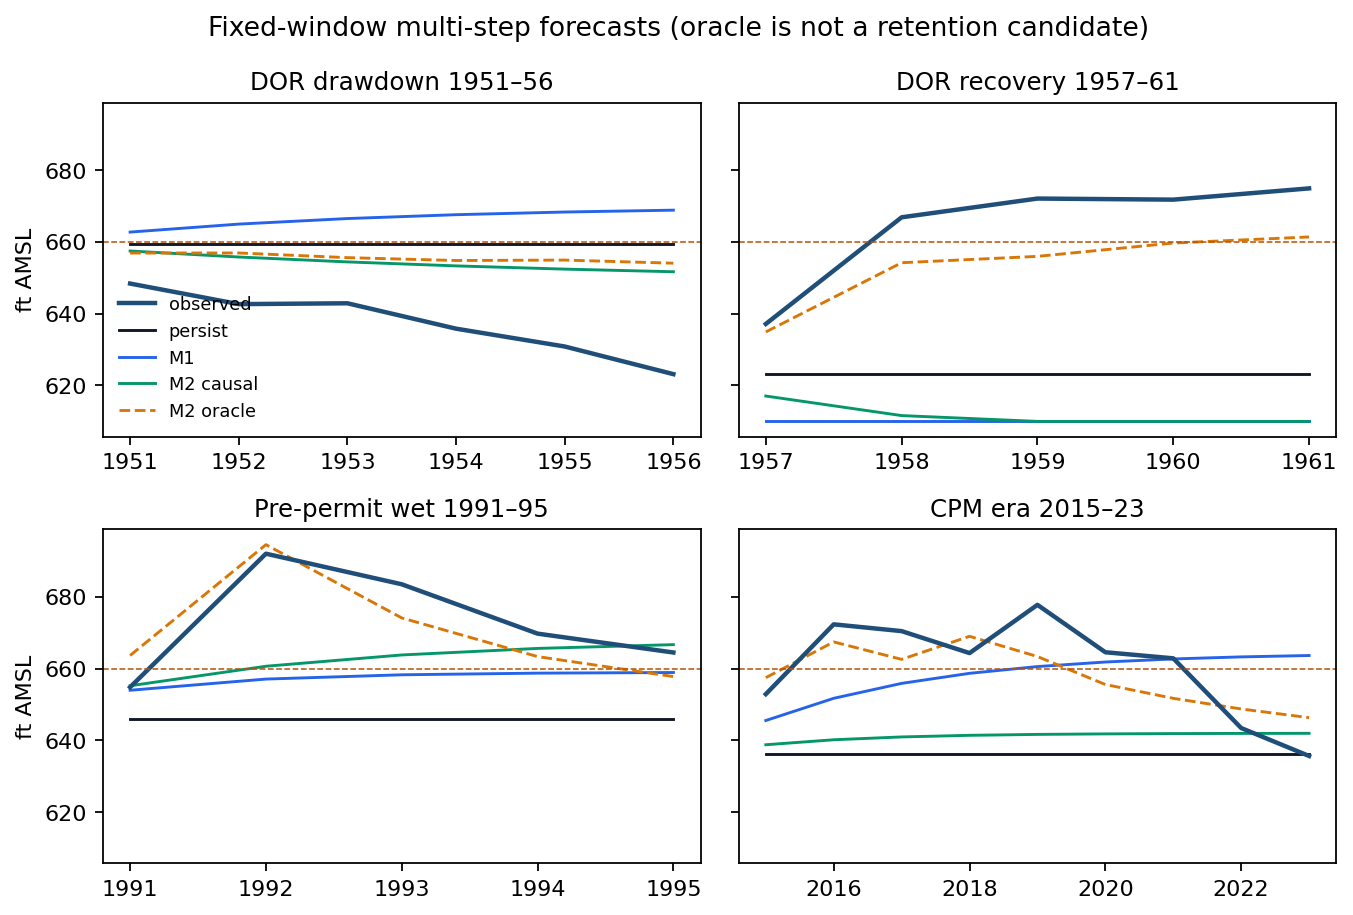
\includegraphics[width=\textwidth]{edw_fig2_windows}
\caption{J-17 multi-step forecasts from the end of each training window. The oracle (dashed) is diagnostic and uses realised future $R,P$.}
\label{fig:si_edwwindows}
\end{figure}

\FloatBarrier
\section{Uncertainty layer: two implementations}\label{si:edwuncertainty}

The post-freeze uncertainty layer (\texttt{e3\_audit\_uncertainty.py}; seed 20260905) attaches Diebold--Mariano tests (Newey--West HAC, lag $h-1$) and moving-block bootstrap intervals (block length 8, 10\,000 replications) to every load-bearing margin, computed from the archived per-origin forecast files; main-text Table~8 reproduces its output. An independent replication (\texttt{campaign\_e3\_dm\_uncertainty.py}, archived with its output \texttt{e3\_dm\_uncertainty.csv}) is a second implementation reading the same registered per-origin forecast file: HAC lag $h-1$ with unweighted truncation and population-variance scaling, block length $h$, 20\,000 replications, seed 0, deterministic (byte-identical on re-execution). Its verified output reproduces every load-bearing reading: the M1 retention margin has DM $z=-0.86$ with block interval $[-1.22,+0.56]$\,ft (bootstrap $p=0.38$); the M2m edge over persistence has $p=0.001$; the $h=5$ climatology win has $p=0.035$. It also registers two rows the main table does not carry, the $h=1$ climatology loss ($+2.94$\,ft against persistence, $p=0.046$) and the M2 $h=5$ loss ($+12.4$\,ft, $p<0.001$), both consistent with the readings above. The two implementations use different seeds, block lengths, HAC weighting and variance conventions, and agree on every conclusion: the 0.39-ft AR(1) retention margin is statistically indistinguishable from zero, the M2m edge is the only one-year margin that separates from noise, and the five-year climatology win survives.

\section{Threshold indicator scores on the post-2007 origins}\label{si:edwbrier}

The second secondary score is scoped to the post-2007 origins, where the 660-ft Stage~I rule is in force. On those origins ($n=16$ at $h=1$) the committed records give 660-ft Brier scores of 0.31 (persistence), 0.25 (M1), 0.25 (M2m), 0.19 (oracle), with the one-year RMSE ranking unchanged (persistence 13.09, M1 12.16, M2m 12.18, M2 13.31, oracle 8.03\,ft); at $h=5$ ($n=12$) the M1--persistence ordering reverses on the subsample (17.16 against 25.10\,ft) and the training mean scores 16.41\,ft, reported without changing the one-year retention statement. For deterministic 0/1 forecasts the Brier score is a misclassification rate of a coarse annual-mean proxy for the Authority's 10-day rule on a small subsample; the full record is archived as \texttt{wave\_e\_edwards/results/rolling\_modern\_2007.csv}.

\FloatBarrier
\section{The service series after the retention freeze}\label{si:edwcomal}

The map $Q=c_0+c_1H$ fitted on 1934--1950 ($c_0=-2876$, $c_1=4.77$) is a linear channel of the same state indexed by J-17; the full-sample contemporaneous correlation is $r=0.986$ (Fig.~\ref{fig:si_edwfibre}). The channel fails in the drought tail, and the direction matters: at the 1956 annual mean (623.15\,ft) it reads $\approx97$\,cfs against an observed $\approx32$\,cfs annual mean, so it predicts non-cessation, and its zero-discharge level ($2876/4.77\approx602.9$\,ft) lies below every observed head (daily minimum 612.5\,ft), so the map never predicts cessation where cessation occurred. Near-linear at ordinary heads, the channel fails at cessation exactly where management cares. One-year Comal RMSE (cfs), scoring the same ladder directly on the Comal series over the same rolling origins ($n=75$): persist 71.9, M1 69.0, M2m 68.7, M2 74.8, M3 73.8, M4 73.4, train-mean 89.7, oracle 45.3; the ranking mirrors the head ranking, as it must for a linear channel. The service series does not change retention, and it cannot: Comal is an independent measurement (a USGS spring gauge, not used to construct J-17) but not an independent information source.

\begin{figure}[!htb]
\centering
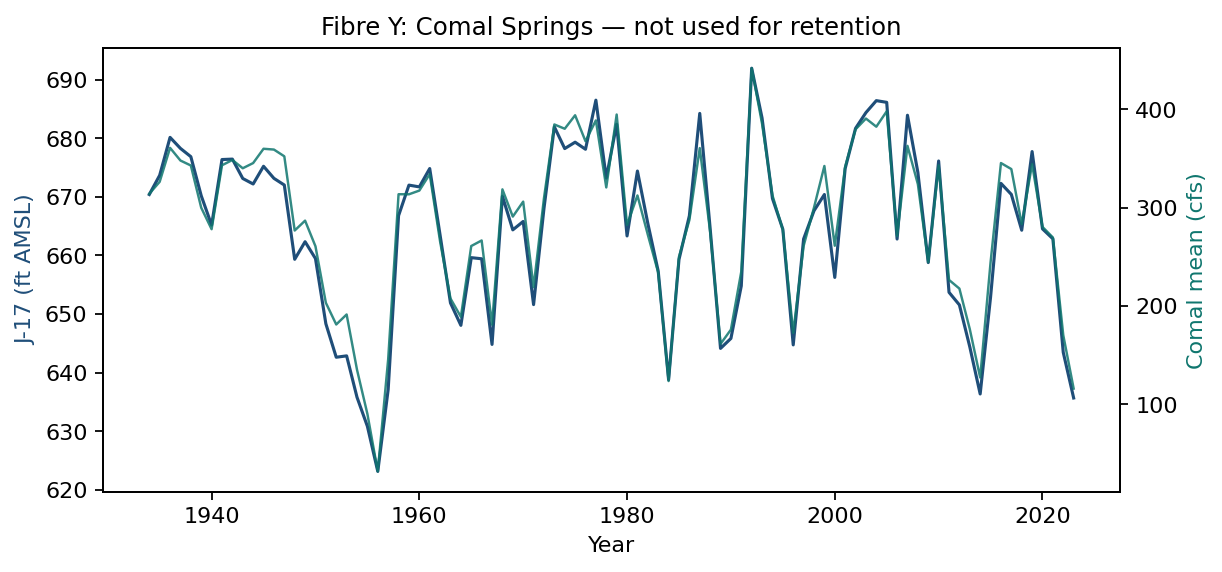
\includegraphics[width=0.85\textwidth]{edw_fig5_fibre}
\caption{Comal annual mean against J-17. Contemporaneous $r=0.986$. The service series is a measured rating curve of the same state.}
\label{fig:si_edwfibre}
\end{figure}

\FloatBarrier
\section{Pumpage counterfactuals}\label{si:edwpumpage}

A declared scenario layer passes counterfactual pumpage paths through the pre-permit affine map (train 1980--1990, the ladder's window~3; the short-window identification caveat applies to the map itself), from the observed 1990 head (645.8\,ft) over 1991--2023 with the actual recharge sequence (Table~\ref{tab:si_pumpage}). The scenarios are counterfactual simulations of the fitted map, not forecasts, and carry no retention implication. Four readings follow. First, pumpage is a secondary lever in this map: the full spread of counterfactual policies spans 630.9--646.8\,ft at 2023, and the map's own RMSE against the observed record (7.2--14.2\,ft) is of the same order as the policy spread, so the 5-ft effects are within model error and are not policy estimates. Second, the 20\%-cut path is the closest to the observed record of the four scenarios (7.19 against 8.56\,ft), an artefact of the map running high on this window (the actual-pumpage path ends 5.9\,ft above the observed 2023 head of 635.7\,ft), not evidence that the Authority's pumpage was near-optimal. Third, the direction is right and the magnitude modest: the 20\% cut raises the simulated 2023 head by 5.2\,ft relative to the actual-pumpage path. Fourth, the recharge coefficient dominates the map through its range, not its magnitude: a $1000\times10^3$ acre-ft recharge difference moves the head by roughly 17.5\,ft at the pre-permit coefficient ($\hat\beta\approx0.0175$; the pumpage coefficient on that train is $-0.031$\,ft per $10^3$ acre-ft, larger per unit but acting on a range of $\sim$300--540 against recharge's 44--2\,486), and $\gamma$ is an ordinary-least-squares association the paper itself diagnoses as simultaneity-contaminated (S17), not a policy lever. The full-sample coefficients $(\hat\beta,\hat\gamma)=(0.017,-0.026)$ differ from the pre-permit window's because the windows differ.

\begin{table}[!htb]
\centering\footnotesize\setlength{\tabcolsep}{3.5pt}
\caption{Pumpage counterfactuals, 1991--2023 (fitted pre-permit map; actual recharge). Pumpage: 1991--2023 mean in $10^3$ acre-ft\,yr$^{-1}$; heads, minimum head over the path and RMSE against the observed record in ft. The observed 2023 head is 635.7\,ft.}
\label{tab:si_pumpage}
\begin{tabular}{@{}lrrrr@{}}
\toprule
Scenario & pumpage & head 2023 & min.\ head & RMSE \\
\midrule
actual pumpage & 382.1 & 641.6 & 640.2 & 8.56 \\
pumpage frozen at 1990 & 489.4 & 630.9 & 630.5 & 14.22 \\
pre-permit mean pumpage & 469.8 & 632.4 & 632.0 & 13.02 \\
20\% pumpage cut & 305.7 & 646.8 & 645.5 & \textbf{7.19} \\
\bottomrule
\end{tabular}
\end{table}

\FloatBarrier
\section{Climate-informed recharge: fixed windows, the recharge target, and the Uvalde note}\label{si:edwclimate}

Fig.~\ref{fig:si_edwpass2} shows the rolling climate-pass scores of main-text Table~9. Same-year corr($R$, precipitation) $=0.78$, which is why the precipitation oracle reduces head RMSE to 10.56\,ft; it remains worse than the full $(R,P)$ oracle (7.55\,ft) because the linear rain map misses 1957-scale extremes. On the 1957--61 recovery no causal climate-informed module has lower RMSE than persistence (persist 43.6\,ft; best causal 48.8\,ft; precipitation oracle 33.7\,ft); September--November 1956 is La Ni\~na ($-0.92$) and does not announce $R_{1957}=1143$. The remaining fixed windows complete the record: drawdown 1951--56, M2\_Renso 24.30, M2\_Rprecip 28.67, M2\_combo 24.70, M2\_Rar 31.38, precipitation oracle 18.16\,ft; pre-permit wet 1991--95, M2\_Rprecip 22.03, M2\_Renso 23.03, M2\_Rar 23.94, M2\_combo 25.71, oracle 10.98\,ft; critical-period era 2015--23, M2\_Rprecip 14.52, M2\_Rar 14.67, M2\_Renso 16.01, M2\_combo 16.57, oracle 9.75\,ft; on this one window the two climate-informed modules M2\_Rprecip and M2\_Rar edge past M1 by about one foot (14.52 and 14.67 against 15.62\,ft). On the recharge target itself the fixed-window scores are an order of magnitude coarser on every window (climate modules 199--937; precipitation oracle 80.7--487, against the $556\times10^3$ acre-ft climatology scale of the rolling record), so the marginal head advantage is a window-specific result, not a recharge forecast. Additional climate indices (PDO, AMO) were not run; they would enter through the same one-step recharge forecast and cannot alter the timing result. A mid-year nowcast would require a new evaluation protocol.

\begin{figure}[!htb]
\centering
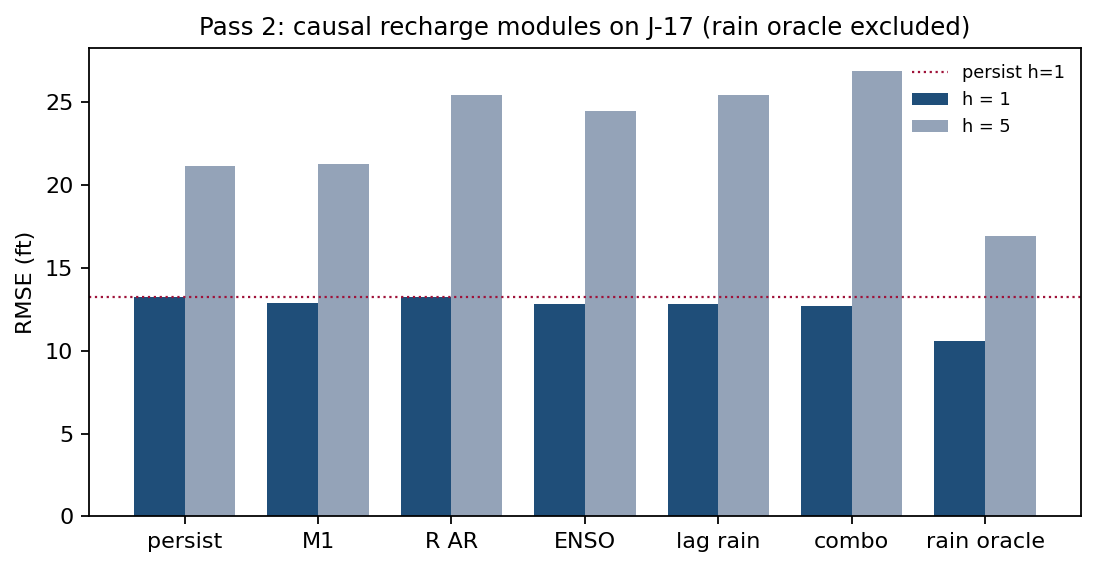
\includegraphics[width=0.85\textwidth]{edw_fig4_pass2}
\caption{Rolling RMSE on J-17 for climate-informed recharge. The precipitation oracle uses year $t+h$ precipitation and cannot be retained.}
\label{fig:si_edwpass2}
\end{figure}

\paragraph{The Uvalde note} An exploratory port of the ladder to the separately regulated Uvalde Pool of the same aquifer (index well J-27; annual head lag-one autocorrelation 0.84) finds the AR(1) losing to persistence by 0.13\,ft at $h=1$, consistent with the direction stated in main-text Section~4.7: on a more strongly autocorrelated head record the AR(1)'s edge over persistence should be smaller. A single additional pool is a direction, not a test; no Uvalde result enters any retention verdict, the two records are not pooled, and the comparison is not offered as a test of anything claimed in the main text.
\FloatBarrier
\part*{Part C: Cross-system material}
\addcontentsline{toc}{part}{Part C: Cross-system material}

\section{Horizon profiles of the baselines and the autocorrelations of Section 5}\label{si:horizon}

Table~\ref{tab:si_horizon} gives the rolling-origin RMSE of last-value persistence and of the training mean at every horizon $h=1,\dots,5$ on the three scored series, computed from the registered data files on the origin sets of the scored ladders (first origin 1990 with an 8-year minimum training window on Specification A; 1965 with 12 years on Specification B; 1948 with 15 years on J-17), together with the lag-$h$ autocorrelation $\rho_h$ of the predictand over the full series and the stationary prediction $\sqrt{2(1-\rho_h)}$ of main-text Remark~2 for the ratio of the two RMSEs. The $h=1$ and $h=5$ values reproduce the archived summaries (main-text Tables~3 and 7) to the printed precision: 98.0/264.7 and 423.6/507.4\,kt on Specification A, 84.4/300.0 and 458.1/521.6\,kt on Specification B, 13.23/21.11 and 16.17/16.80\,ft on J-17. On J-17 the observed ratio tracks the prediction within 0.11 at every horizon, always from below, and crosses one between $h=1$ and $h=2$, where $\rho_h$ falls through one half. On both cod series the observed ratio stays far below the prediction at every horizon, the training mean of a collapsing series being a poor forecast of anything; the stationary formula would place a crossover between four and five years on Specification A and beyond five on Specification B, and neither occurs. The script is \texttt{work/horizon\_profile.py}; its JSON summary is archived beside it.

\begin{table}[!htb]
\centering\footnotesize\setlength{\tabcolsep}{3.5pt}
\caption{Horizon profile of the two baselines on the scored origin sets. RMSE in kt (cod) and ft (J-17); ratio $=$ RMSE(persistence)/RMSE(training mean); $\rho_h$ is the lag-$h$ autocorrelation of the predictand over the full series.}
\label{tab:si_horizon}
\resizebox{\textwidth}{!}{%
\begin{tabular}{@{}lrrrrrrr@{}}
\toprule
Series & $h$ & $n$ & persist & mean & ratio & $\rho_h$ & $\sqrt{2(1-\rho_h)}$ \\
\midrule
J-17 head (ft) & 1 & 75 & 13.23 & 16.17 & 0.818 & 0.629 & 0.861 \\
 & 2 & 74 & 17.69 & 16.58 & 1.067 & 0.348 & 1.142 \\
 & 3 & 73 & 20.59 & 16.88 & 1.220 & 0.137 & 1.314 \\
 & 4 & 72 & 21.50 & 16.93 & 1.270 & 0.061 & 1.371 \\
 & 5 & 71 & 21.11 & 16.80 & 1.256 & 0.073 & 1.361 \\
\midrule
Cod A, SSB (kt) & 1 & 25 & 98.05 & 423.59 & 0.231 & 0.933 & 0.365 \\
 & 2 & 24 & 184.32 & 460.54 & 0.400 & 0.825 & 0.592 \\
 & 3 & 23 & 237.97 & 488.07 & 0.488 & 0.687 & 0.792 \\
 & 4 & 22 & 256.74 & 500.18 & 0.513 & 0.553 & 0.945 \\
 & 5 & 21 & 264.72 & 507.39 & 0.522 & 0.406 & 1.090 \\
\midrule
Cod B, SSB (kt) & 1 & 59 & 84.43 & 458.12 & 0.184 & 0.971 & 0.241 \\
 & 2 & 58 & 152.44 & 474.51 & 0.321 & 0.913 & 0.417 \\
 & 3 & 57 & 208.89 & 489.99 & 0.426 & 0.838 & 0.569 \\
 & 4 & 56 & 258.77 & 505.80 & 0.512 & 0.757 & 0.697 \\
 & 5 & 55 & 299.98 & 521.56 & 0.575 & 0.678 & 0.802 \\
\bottomrule
\end{tabular}}

\end{table}

Table~\ref{tab:si_autocorr} gives the lag-one autocorrelations, means and standard deviations used in main-text Section~5.1. The J-17 flux mechanism is $\hat\beta R_t+\hat\gamma P_t$ with the full-sample least-squares coefficients of the one-pool map, $(\hat\alpha,\hat\beta,\hat\gamma,\hat\delta)=(177.6,\,0.0173,\,-0.0260,\,-0.273)$; the apparent net production of the cod series is $S_{t+1}-S_t+C_t$ with the catch series of the respective pass. The stylised prediction of Proposition~2(ii) for J-17 uses $\sigma^2=84.6$\,ft$^2$ and $\rho=0.078$, giving $\sigma^2(1-2\rho)=71.4$\,ft$^2$, a predicted one-year M2 RMSE of $\sqrt{13.23^2+71.4}=15.70$\,ft against the archived 14.70\,ft, and a predicted M2m-over-M2 mean-square advantage of 71.4\,ft$^2$ against the archived $14.70^2-12.28^2=65.1$\,ft$^2$. Further correlations used in the main text: $r(\Delta H_t,R_t)=0.742$, $r(\Delta H_t,R_{t-1})=0.056$, $r(R_t,R_{t-1})=0.172$ as a Pearson correlation of successive pairs (0.170 as the autocovariance-based estimator in the table), and $r(H_t,H_{t-1})=0.644$ as a Pearson correlation of pairs (0.629 autocovariance-based; the single-system aquifer study quoted 0.64).

\begin{table}[!htb]
\centering\footnotesize\setlength{\tabcolsep}{3.5pt}
\caption{Lag-one autocorrelations (autocovariance estimator), means and standard deviations of the series used in main-text Section~5.1. Units: ft and $10^3$ acre-ft for J-17; kt for cod.}
\label{tab:si_autocorr}
\begin{tabular}{@{}lrrr@{}}
\toprule
Series & $\rho_1$ & mean & s.d. \\
\midrule
J-17: annual recharge $R_t$ & 0.170 & 682.83 & 515.44 \\
J-17: annual pumpage $P_t$ & 0.870 & 318.82 & 114.41 \\
J-17: flux mechanism $\hat\beta R_t+\hat\gamma P_t$ & 0.078 & 3.52 & 9.20 \\
J-17: head increment $\Delta H_t$ & -0.115 & -0.39 & 12.34 \\
J-17: head $H_t$ & 0.629 & 664.42 & 14.70 \\
Cod A: apparent net production, coarse regime & 0.753 & 57.74 & 112.71 \\
Cod A: apparent net production, annual landings & 0.714 & 53.00 & 124.86 \\
Cod B: apparent net production, landings & 0.908 & 184.73 & 212.65 \\
Cod A: SSB $S_t$ & 0.933 & 300.51 & 356.51 \\
Cod B: SSB $S_t$ & 0.971 & 512.76 & 423.25 \\
\bottomrule
\end{tabular}
\end{table}

\section{Verification record for this edition}\label{si:verify}

The verification script \texttt{paper11\_forecasting\_\allowbreak{}baselines\_v67\_\allowbreak{}verification.py} (standard library only) reads the registered data files and archived result files of both systems together with the manuscript sources (main text and this document) and asserts, in order: (a) the cod outcome-year, vintage and threshold cross-checks carried over from the single-system edition (S10--S12), including the presence of every pinned value in the sources; (b) every cell of main-text Tables~7--9 against \texttt{wave\_e\_edwards/results/rolling\_summary.csv}, \texttt{pass2\_H\_summary.csv}, \texttt{pass2\_R\_summary.csv} and \texttt{e3\_audit\_uncertainty.json}, the fixed-window cells of S17 against \texttt{fixed\_window\_scores.csv}, the post-2007 record of S19 against \texttt{rolling\_modern\_2007.csv} and the Comal ranking of S20 against \texttt{fibre\_comal\_summary.csv}; (c) the baseline horizon profile of S23 recomputed from the registered series, its agreement with the archived $h=1$ and $h=5$ summaries of both systems, and the autocorrelations quoted in Section~5; (d) the arithmetic of Proposition~2 on the J-17 numbers (the sign of $\sigma^2(1-2\rho)-\mu^2$, the predicted ordering M2m $\le$ persist $<$ M2, and the agreement of the predicted M2m-over-M2 advantage with the archived one to within 10\%); and (e) textual invariants (no claim of prospective registration; the two protocols stated with their disclosed completions; the retraction of the ``weakly autocorrelated surplus production'' reading accompanied by the computed value). The run for this edition reports 139 checks passing and none failing; its output is archived beside the script.

\end{document}
